\documentclass[11pt]{article}

% ============================================================
% main.tex --- Neutrino theory chapter (PhD thesis).
% Sections live in sections/. Bibliography in main.bib.
% Build output: build/main.pdf (plan/ is a separate document).
%
% This compiles standalone for drafting. When integrated into the
% full thesis, replace \documentclass{article} with \chapter{} and
% drop the preamble.
% ============================================================

% ---- Geometry & typography -------------------------------------------------
\usepackage[margin=1in]{geometry}
\usepackage{microtype}
\usepackage{setspace}
\setstretch{1.15}

% ---- Maths -----------------------------------------------------------------
\usepackage{amsmath, amssymb}
% Number equations as (section.subsection.n), resetting each subsection.
% Equations outside any subsection get (section.0.n).
\numberwithin{equation}{subsection}
% Lightweight stand-ins (TeX Live basic lacks braket/dsfont)
\newcommand{\ket}[1]{\lvert #1 \rangle}
\newcommand{\bra}[1]{\langle #1 \rvert}
\newcommand{\braket}[2]{\langle #1 | #2 \rangle}
\newcommand{\mathds}[1]{\mathbb{#1}}

% ---- Figures & tables ------------------------------------------------------
\usepackage{graphicx}
\graphicspath{{images/}}
\usepackage{subcaption}
\usepackage{booktabs}
\usepackage{xcolor}

% ---- Bibliography ----------------------------------------------------------
\usepackage[numbers,square,sort&compress]{natbib}

% ---- Headers ---------------------------------------------------------------
\usepackage{fancyhdr}
\pagestyle{fancy}
\fancyhf{}
\fancyhead[L]{\leftmark}
\fancyhead[R]{\thepage}
\renewcommand{\headrulewidth}{0.4pt}

% ---- Hyperlinks (load last) -----------------------------------------------
\usepackage[hidelinks]{hyperref}

% ---- Local shortcuts -------------------------------------------------------
\newcommand{\numu}{\nu_\mu}
\newcommand{\nue}{\nu_e}
\newcommand{\nutau}{\nu_\tau}
\newcommand{\numubar}{\bar\nu_\mu}
\newcommand{\nuebar}{\bar\nu_e}
\newcommand{\dm}[1]{\Delta m^{2}_{#1}}
\newcommand{\dcp}{\delta_{\rm CP}}
\newcommand{\PMNS}{U_{\rm PMNS}}

% ---- Title -----------------------------------------------------------------
\title{Neutrino Theory}
\author{Oscar Chow}
\date{}

% ============================================================================
\begin{document}
\maketitle

\section*{Declaration}
This chapter is submitted as part of my third year progression. The physics, arguments, and final wording are my own.

Generative AI was used to help write the Python script for the two-flavour survival figure (Fig.~\ref{fig:two-flavour-survival-probability}) and the drawing code for the mass-ordering schematic (Fig.~\ref{fig:mass-ordering}). It was also used to check grammar and to rephrase some sentences. I take responsibility for the chapter as submitted.

\tableofcontents
\clearpage

% !TEX root = ../main.tex
Neutrinos are elementary particles of the Standard Model (SM). They are electrically neutral leptons that come 
in three flavours, corresponding to the electron, muon and tau charged leptons. Neutrinos have been observed to oscillate or change between these flavours as they propagate, a fact that implies that neutrinos, contrary to the SM prediction, are massive. This chapter begins with a brief history of the neutrino, from its postulate to the discovery of the three flavours and the observation of oscillations. It then places the neutrino in the SM, developing the theory of flavour mixing and oscillations, and reviews the experimental landscape, including three remaining open questions, namely, the mass ordering, the octant of $\theta_{23}$, and the value of $\dcp$.

\section{A Brief History of the Neutrino}
\label{sec:history}

\subsection{The Neutrino Postulate}

By the early 20th century, decay products of atomic nuclei were understood to produce discrete energy spectra. 
This behaviour was observed in both $\alpha$- and $\gamma$-decays:
\begin{align}
    {}^{A}_{Z}X &\rightarrow {}^{A-4}_{Z-2}Y + {}^{4}_{2}\mathrm{\alpha},
    \label{eq:alpha-decay} \\
    {}^{A}_{Z}X^{*} &\rightarrow {}^{A}_{Z}X + \gamma.
    \label{eq:gamma-decay}
\end{align}
In $\alpha$-decay (Eq.~\ref{eq:alpha-decay}), the fixed energy of the emitted $\alpha$ particle is determined by the two-body kinematics of the decay process.
Similarly, the discrete energy spectrum of $\gamma$-decay (Eq.~\ref{eq:gamma-decay}) arises from the de-excitation of the nucleus to a lower energy state, where the difference between the two energy levels corresponds to the emitted photon energy.
This understanding therefore left James Chadwick puzzled when he discovered, in 1914, that the energy spectrum of the emitted electron in $\beta$-decay, then assumed to be the two-body process
\begin{equation}
    {}^{A}_{Z}X \rightarrow {}^{A}_{Z+1}Y + e^{-},
    \label{eq:beta-decay}
\end{equation}
was continuous~\cite{Chadwick1914,Zuber2020}.
The implications of this observation were only addressed in 1930 by Wolfgang Pauli, who proposed that there must be another neutral particle in the final state, so that $\beta$-decay proceeds as
\begin{equation}
    {}^{A}_{Z}X \rightarrow {}^{A}_{Z+1}Y + e^{-} + \bar{\nu}_e.
    \label{eq:beta-decay-threebody}
\end{equation}
In addition to resolving the apparent violation of energy conservation, Pauli's postulate also provided a solution to the fact that the decay could not just emit one spin-$\frac{1}{2}$ particle (a fermion), but must emit another.
Pauli provisionally named this neutral fermion the neutron; it was later renamed the neutrino by Fermi. 

\subsection{First Direct Neutrino Detection and Discovery}
The first direct detection of the electron antineutrino was made in 1956 by Clyde Cowan and Frederick Reines~\cite{ReinesCowan1953,CowanReines1956}.
They used a water tank and layers of liquid scintillators, placed near a nuclear reactor, which provided a large antineutrino flux.
An incoming antineutrino interacting with a proton produces a neutron and a positron via inverse beta decay:
\begin{equation}
    p + \overline{\nu}_e \rightarrow n + e^{+}.
    \label{eq:inverse-beta-decay}
\end{equation}
Two gamma rays are produced when the positron annihilates with an
electron. The detection of these gammas, followed shortly (a few
$\mu$s) by detection of the neutron capture photon, provided a clear
signal of the neutrino-proton interaction.
Reines was awarded the Nobel Prize in Physics in 1995 for the discovery of the electron antineutrino.

\subsection{$\nu_{\mu}$ and $\nu_{\tau}$ Discovery}
Further to Reines and Cowan's discovery, it was understood that reactor and $\beta$-decay neutrinos were associated with an electron (or a $\beta$ particle)~\cite{CowanReines1956} (Eq.~\ref{eq:inverse-beta-decay}). 
In contrast, the question remained as to whether the neutrino resulting from pion decay, produced alongside a muon, was the same neutrino as that of $\beta$-decay~\cite{Feinberg1958,Pontecorvo1960}. 
To answer this, in 1962 Lederman, Schwartz, Steinberger and collaborators at Brookhaven National Laboratory used the world's first accelerator-based neutrino beam~\cite{Danby1962}. 
Accelerated protons were collided with a target to produce pions, which subsequently
decayed to produce muons and neutrinos. 
The resulting neutrinos were detected, and the interactions were found to produce muons rather than electrons. 
This led to the conclusion that there must be at least two types of
neutrinos: those associated with electrons (reactor and $\beta$-decay)
and those associated with muons (pion decay).
Lederman, Schwartz and Steinberger were awarded the 1988 Nobel Prize in Physics for the discovery of the muon neutrino.

When the tau lepton was discovered in 1975~\cite{Perl1975}, a third associated tau neutrino was expected. 
The Direct Observation of the Nu Tau (DONUT) experiment at Fermilab successfully observed it in 2000~\cite{Kodama2001}. 
This completed the direct observation of the three Standard Model (SM) neutrino flavours.

\subsection{Solar and Atmospheric Anomalies}
\label{sec:history-anomalies}
In parallel to the direct observation of the neutrino, Bruno Pontecorvo theorised in 1957 that neutrinos, like neutral kaons, could oscillate.
This was the first suggestion of neutrino oscillations, but in contrast to today's knowledge, and in analogy with the neutral kaon system ($K^0\leftrightarrow\bar{K}^0$), these oscillations were between neutrinos and antineutrinos~\cite{Pontecorvo1957,Pontecorvo1958}.
In 1962, following the muon neutrino discovery, Maki, Nakagawa and Sakata adapted Pontecorvo's proposal by postulating that the muon and electron neutrinos could mix, the first flavour mixing formulation.
This was further developed by Pontecorvo in 1967, who returned to the problem, formulating two neutrino flavour oscillations~\cite{MakiNakagawaSakata1962,Pontecorvo1967} and suggesting that such oscillations would reduce the solar neutrino flux observed on Earth.
Two and three flavour oscillations will be discussed in more detail in Sec.~\ref{sec:oscillations}.

The following year, Ray Davis and collaborators conducted the Homestake experiment, which used a 615 tonne tank of liquid perchloroethylene deep underground to detect solar neutrinos via the reaction: $\nu_{e} + {}^{37}\mathrm{Cl} \rightarrow {}^{37}\mathrm{Ar} + e^{-}$~\cite{Davis1968,Miramonti2009}.
The measured rate of solar neutrinos was found to be significantly lower than that predicted by the Standard Solar Model (SSM).
This discrepancy was known as the \emph{Solar Neutrino Problem}.
Although neutrino oscillations had already been proposed in the previous year, they were not widely accepted as an explanation for this discrepancy.
The solar neutrino deficit was later confirmed by the Kamiokande, SAGE and GALLEX experiments~\cite{Hirata1990,Abazov1991,Anselmann1992}.

A second discrepancy emerged from the measurement of the atmospheric neutrino flux.
These neutrinos are produced when cosmic rays interact with Earth's
atmosphere, producing charged pions and kaons, which subsequently decay
into muons and muon neutrinos. The muons eventually also decay into
electrons, muon neutrinos and electron neutrinos.
The observed muon neutrino flux was lower than expected.
In 1998, the Super-Kamiokande experiment (SK) reported that this deficit exhibited a dependence on the zenith angle, and therefore the distance travelled by the neutrinos through the Earth.
This path length dependence was the first compelling evidence for neutrino oscillations~\cite{Fukuda1998}.

In 2002, the Sudbury Neutrino Observatory (SNO) showed that the total solar neutrino flux was consistent with the SSM, while showing the same electron neutrino flux as previous experiments claiming a deficit.
The total solar neutrino flux was measured via the neutral-current (NC)
interaction, which does not allow for flavour determination and occurs
for all flavours, while the electron neutrino flux was measured via the
charged-current (CC) interaction by measuring the final-state electron.
This suggested that solar electron neutrinos must have undergone flavour transformation as they travelled through the Sun and to the Earth, hence resolving the Solar Neutrino Problem~\cite{Ahmad2002}.
The full interpretation of the SNO result also requires the matter effect, which will be introduced in Sec.~\ref{sec:matter}.



% !TEX root = ../main.tex
\section{Neutrinos in the Standard Model}
\label{sec:sm}

The previous section discussed several experimental discoveries of different neutrino types, or flavours, and concluded that they should transform as they travel. To understand why this fact is so important, we must motivate how the neutrino enters the Standard Model (SM), describe how it behaves in this theory, and explain what is meant by different neutrino flavours. This brief section follows Refs.~\cite{CottinghamGreenwood2007,Thomson2013,Zuber2020}.

Neutrinos enter the SM as neutral leptons, and there exists a flavour for each of the charged leptons: the electron, muon and tau neutrinos, corresponding to the electron, muon and tau. They carry neither electric nor colour charge, meaning they only couple to the weak interaction, and therefore can only be produced, and only interact, via the weak force. As briefly mentioned above, there are many sources of neutrinos that can be measured on Earth; these include stellar, supernovae and cosmic ray sources, as well as particle accelerators and fission reactors. Since the weak force has weak coupling, the vast majority of these neutrinos pass through matter without interacting.

There are two neutrino interaction types in the SM; charged-current (CC) and neutral-current (NC). The vertices for such interactions can be described by the current:
\begin{equation}
    J^{\mu}\sim\overline{u}(p')\,\gamma^{\mu}\tfrac{1}{2}\left(1-\gamma^{5}\right)u(p),
    \label{eq:charged-current}
\end{equation}
where $u(p)$ and $\overline{u}(p')$ are Dirac spinors representing the incoming and outgoing fermions, $\overline{u}=u^{\dagger}\gamma^{0}$ is the Dirac adjoint, and the $\gamma^{\mu}$ are the Dirac matrices. Expanding this gives a $\frac{1}{2}\overline{u}(p')\gamma^{\mu}u(p)$ term, which is the vector current, and a $\frac{1}{2}\overline{u}(p')\gamma^{\mu}\gamma^{5}u(p)$ term, which is the axial-vector current. This is a vector minus axial-vector combination, that violates parity maximally\footnote{Under parity, the vector and axial-vector components transform oppositely. The relative sign between them flips and V$-$A is mapped to V$+$A. In the Lagrangian, the $V^{2}$ and $A^{2}$ contraction terms are unchanged but the $V\cdot A$ term reverses sign. With this extra term, the Lagrangian describes a different theory after the transformation, and parity is therefore violated. The interference term is as large as it can be, so parity is maximally violated.}.
The factor $\tfrac{1}{2}\left(1-\gamma^{5}\right)$ is exactly the left-handed chiral projection operator $P_{L}$, which projects out the left-handed chiral components of the field. As a result, only left-handed chiral particles and right-handed chiral antiparticles take part in the weak interaction.

The electroweak unification into an $SU(2)_{L}\times U(1)_{Y}$~\cite{Weinberg1967} gauge theory gives rise to two physical charged gauge bosons, $W^{\pm}$, which mediate CC interactions, and a neutral gauge boson, $Z^{0}$, which mediates NC interactions. The massless photon, $A^{0}$ also emerges from this unification. Figure~\ref{fig:sm-vertices} shows the vertices for CC and NC interactions. Comparing these vertices shows that CC interactions have a final-state charged lepton with flavour matching that of the incoming neutrino. Measuring this charged lepton from CC interactions therefore allows for the identification of the flavour of the incoming neutrino. NC interactions, on the other hand, have no such final-state charged lepton, and therefore cannot determine the flavour of the incoming neutrino.

\begin{figure}[htbp]
    \centering
    \begin{subfigure}[b]{0.46\textwidth}
        \centering
        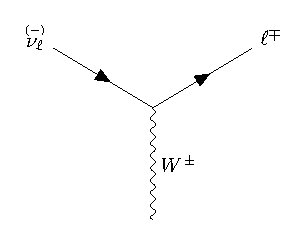
\includegraphics[width=\linewidth]{feyn_cc_vertex.pdf}
        \caption{Charged current}
        \label{fig:cc-vertex}
    \end{subfigure}
    \hfill
    \begin{subfigure}[b]{0.46\textwidth}
        \centering
        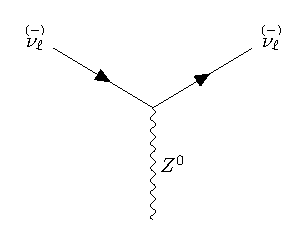
\includegraphics[width=\linewidth]{feyn_nc_vertex.pdf}
        \caption{Neutral current}
        \label{fig:nc-vertex}
    \end{subfigure}
    \caption{Feynman diagrams showing the two neutrino interaction types (as leptonic vertices), with
    time flowing from left to right and $\ell=e,\mu,\tau$. (a) shows a CC interaction, in which the
    incoming (anti)neutrino is converted into its corresponding charged lepton, mediated by a
    $W^{\pm}$ boson. (b) shows a NC interaction, mediated by a $Z^{0}$, in which the neutrino
    remains in the final state, so the flavour of the incoming neutrino cannot be known.
    Adapted from Ref.~\cite{Booth2021}.}
    \label{fig:sm-vertices}
\end{figure}


% !TEX root = ../main.tex
\section{Neutrino Mixing and Oscillations}
\label{sec:oscillations}


The flavour of a neutrino denotes its state when it is produced of detected. It was previously mentioned that neutrinos oscillate, or change flavour as they propagate. This statement suggests that at one point in time, a neutrino is produced as a given flavour, and at a later point in time, it is detected as a different flavour. This means that a proppagating neutrino experiences and evolves as a funciton of time. This statement is not true for massless particles, as they travel at the speed of light, so no proper time elapses as they travel. Neutrino oscillations therefore, imply that neutrinos are massive.

This section introduces the orthogonal bases that neutrino oscillations (or flavour change) require, namely, flavour and mass eigenstates. 
Section~\ref{sec:two-flavour} begins the oscillation probability derivation for the two-flavour case. Section~\ref{sec:pmns} then introduces how these bases are related by a unitary mixing matrix and gives an overview of the oscillation parameters. This allows for the expansion of the theory to three flavours in Section~\ref{sec:three-flavour}, where the hierarchy of the mass states is also discussed\footnote{An open question that this thesis addresses.}. Section~\ref{sec:matter} then discusses an important effect that arises due to the propagation of neutrinos through the Earth (or more generally, through matter), which modifies the oscillation probability. Although this effect primarily affects the appearance channel, since this thesis is concerned with a disappearance measurement, the emphasis throughout this section is with the $\numu$ survival probability.

\subsection{Flavour and Mass Eigenstates}
\label{sec:flavour-mass}
As mentioned, neutrinos are produced and detected as observable flavour eigenstates of the weak interaction. 
Before they are detected and after they are produced, they must propagate and evolve as a function of time. These evolving states, therefore propagate freely as a particle with definite mass. These mass eigenstates are the states that diagonalise the free particle Hamiltonian. It can be shown that the flavour states are linear combinations of the mass states. Since these form an orthonomal basis set, these two bases are related by a unitary transformation and can be written as:
\begin{equation}
    \ket{\nu_\alpha} = \sum^{N}_{j} U^{*}_{\alpha j}\ket{\nu_j},
    \qquad
    \ket{\nu_j} = \sum^{N}_{\alpha} U_{\alpha j}\ket{\nu_\alpha}.
    \label{eq:mixing-relation}
\end{equation}
$\ket{\nu_\alpha}$ denotes the flavour eigenstates, where $N$ is the number of flavours, and $\ket{\nu_j}$ denotes the mass eigenstates, and $U$ is the unitary mixing matrix, known as the Pontecorvo--Maki--Nakagawa--Sakata (PMNS) matrix, which will be discussed in more detail in Section~\ref{sec:pmns}. in the three-flavour picture, $N=3$, and $\alpha \in \{e,\mu,\tau\}$.
Convention is for $U$ to be conjugated in the first relation. \textcolor{red}{For antineutrinos the roles of $U$ and $U^{*}$ are interchanged, a fact that becomes important when CP violation is discussed in Sec.~\ref{sec:three-flavour}}

Equation~\hyperref[eq:mixing-relation]{(\ref{eq:mixing-relation})} states that a given neutrino flavour state is a coherent superposition of mass states. As these mass states propagate, their relative contributions will evolve, leading to the non-zero probability that the measured flavour state is different to the produced one.

\subsection{Two-Flavour Oscillations}
\label{sec:two-flavour}
The derivation presented below loosely follows that of Refs.~\cite{GiuntiKim2007,Booth2021}.
To derive the two-flavour oscillation mechanism, we first consider the flavour and mass eigenstate mixing relations in Eq.~\hyperref[eq:mixing-relation]{(\ref{eq:mixing-relation})}. To begin, it is useful first, to consider the picture with two flavour states, $\ket{\nu_\alpha}$ and $\ket{\nu_\beta}$, and two mass states, $\ket{\nu_1}$ and $\ket{\nu_2}$, with masses $m_1$ and $m_2$. The unitary mixing matrix $U$ can be express as a $2\times2$ rotation matrix through an angle $\theta$:

\begin{equation}
    \begin{pmatrix} \ket{\nu_\alpha} \\ \ket{\nu_\beta} \end{pmatrix}
    =
    \begin{pmatrix} U^{*}_{\alpha 1} & U^{*}_{\alpha 2} \\ U^{*}_{\beta 1} & U^{*}_{\beta 2} \end{pmatrix}
    \begin{pmatrix} \ket{\nu_1} \\ \ket{\nu_2} \end{pmatrix}
    =
    \begin{pmatrix} \cos\theta & \sin\theta \\ -\sin\theta & \cos\theta \end{pmatrix}
    \begin{pmatrix} \ket{\nu_1} \\ \ket{\nu_2} \end{pmatrix}.
    \label{eq:two-flavour-mixing-matrix}
\end{equation}
Multiplying this out, shows that the flavour states can be written as a linear combination of the mass states, 
\begin{equation}
    \ket{\nu_\alpha} = U^{*}_{\alpha 1}\ket{\nu_1} + U^{*}_{\alpha 2}\ket{\nu_2}
    = \cos\theta \ket{\nu_1} + \sin\theta \ket{\nu_2},
    \qquad
    \ket{\nu_\beta} = U^{*}_{\beta 1}\ket{\nu_1} + U^{*}_{\beta 2}\ket{\nu_2}
    = -\sin\theta \ket{\nu_1} + \cos\theta \ket{\nu_2},
    \label{eq:two-flavour-mixing}
\end{equation}
an idea that will be important when considering how the oscillation probabilities evolve with time.
Next, we reiterate the the neutrino mass states are eigenstates of the free particle Hamiltonian. Therefore, they evolve as a function of time as plane waves; solutions to the time-dependent Schrödinger equation:
\begin{equation}
    i\hbar \frac{\partial}{\partial t} \ket{\nu_j(t,\vec{x})} = - \frac{1}{2m_j} \nabla^2 \ket{\nu_j(t,\vec{x})}.
    \label{eq:time-dependent-schrodinger}
\end{equation}
The plane wave solutions to this equation are of the form:
\begin{equation}
    \ket{\nu_j(t,\vec{x})} = e^{-i(E_j t - \vec{p}_j\cdot\vec{x})/\hbar} \ket{\nu_j(0,\vec{0})},
    \label{eq:plane-wave-solution}
\end{equation}
where $E_j = \sqrt{|\vec{p}_j|^{2} + m_j^{2}}$ is the energy of the $j$th mass state, and $\vec{p}_j$ is its three-momentum.
 
Using the assumption that neutrinos are ultra-relativistic, that is, $m_j \ll E_j$, and by choosing the equal momentum idealisation of the mass states, it can be shown that the energy of the $j$th mass state can be writtten as:
\begin{equation}
    E_j = \sqrt{|\vec{p}_j|^{2} + m_j^{2}} \simeq |\vec{p}_j| + \frac{m_j^{2}}{2|\vec{p}_j|} \simeq E + \frac{m_j^{2}}{2E},
    \label{eq:relativistic-expansion}
\end{equation}
where $E$ is the common leading order energy the states. The ultra-relativistic limit allows us to approximate the time as the propagation distance, $t \simeq L$, when working in natural units. The plane wave exponent, or the phase accumulated therefore becomes:
\begin{equation}
    \phi_j = E_j t - \vec{p}_j\cdot\vec{x} \simeq \frac{m_j^{2}L}{2E}.
    \label{eq:phase}
\end{equation}

Subsequently, one can combine Eq. \hyperref[eq:two-flavour-mixing]{(\ref{eq:two-flavour-mixing})}, Eq. \hyperref[eq:plane-wave-solution]{(\ref{eq:plane-wave-solution})} and Eq. \hyperref[eq:phase]{(\ref{eq:phase})} to write the amplitude for the transition from $\ket{\nu_\alpha}$ to $\ket{\nu_\beta}$ and take the inner product :
\begin{equation}
    A(\nu_\alpha \to \nu_\beta)
    = \braket{\nu_\beta}{\nu_\alpha(L)}
    = -\sin\theta\cos\theta\, e^{-i\phi_1} + \cos\theta\sin\theta\, e^{-i\phi_2}
    = \sin\theta\cos\theta\left(e^{-i\phi_2} - e^{-i\phi_1}\right).
    \label{eq:amplitude}
\end{equation}
By taking the squared modulus of this amplitude, and using the identity $|e^{-i\phi_2}-e^{-i\phi_1}|^{2} = 2 - 2\cos\Delta\phi = 4\sin^{2}(\Delta\phi/2)$, where $\Delta\phi = \phi_2 - \phi_1 = \dm{}L/2E$ with $\dm{} \equiv m_2^{2}-m_1^{2}$, the transition probability becomes:
\begin{equation}
    P(\nu_\alpha \to \nu_\beta)
    = 4\sin^{2}\theta\cos^{2}\theta \sin^{2}\!\left(\frac{\Delta\phi}{2}\right)
    = \sin^{2}(2\theta)\,\sin^{2}\!\left(\frac{\dm{}L}{4E}\right).
    \label{eq:two-flavour-appearance}
\end{equation}
One can also write the survival probability as the complement as we are only considering two flavours, 
\begin{equation}
    P(\nu_\alpha \to \nu_\alpha) = 1 - \sin^{2}(2\theta)\,\sin^{2}\!\left(\frac{\dm{}L}{4E}\right).
    \label{eq:two-flavour-survival}
\end{equation}

Reintroducing $\hbar$ and $c$, and converting quantities into units an experiment would work with, Eq.~\hyperref[eq:two-flavour-survival]{(\ref{eq:two-flavour-survival})} becomes:
\begin{equation}
    P(\nu_\alpha \to \nu_\alpha) = 1 - \sin^{2}(2\theta)\,\sin^{2}\!\left(
        \frac{1.27\,\dm{}[\mathrm{eV}^{2}]\;L[\mathrm{km}]}{E[\mathrm{GeV}]}
    \right).
    \label{eq:two-flavour-practical}
\end{equation}
This expression depends on only two physical parameters, the mixing angle $\theta$ and the mass-squared splitting $\dm{}$. The experiment only has control over the probablity via the ratio $L/E$. The effects of these parameters on the survival probability are shown in Fig.~\ref{fig:two-flavour-survival-probability}, which shows the probability as a function of baseline at a fixed energy as well as a function of energy at a fixed baseline. Both panels show that the amplitude of the survival probability is directly dictated by $\sin^{2}(2\theta)$, and hence the mixing angle, while $\dm{}$ sets the frequency of oscillations in the left panel. In the right panel, the oscillation phase varies as function of $1/E$, and the minima become more closely spaced at lower energies. Conversely, at higher energies, the phase goes to zero resulting in unit survival probability. 

\begin{figure}[htbp]
    \centering
    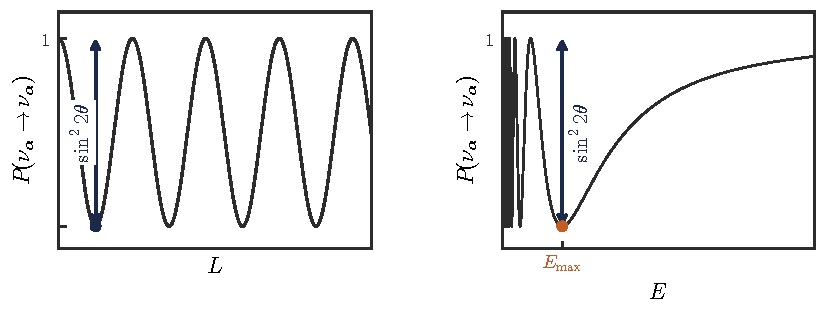
\includegraphics[width=\textwidth]{two_flavour_survival}
    \caption{Two-flavour survival probability as a function of propagation distance at fixed
    energy (\textbf{left}) and of neutrino energy at fixed baseline (\textbf{right}). The mixing
    angle sets the depth of the oscillation through $\sin^{2}(2\theta)$, while $\dm{}$ determines the position of the minima by setting the oscillation phase. Plotting this as a function of energy shows that the variation is not periodic, this is due to the $1/E$ dependence of the phase. The highest-energy minimum lies at $E_{\rm max}$.}
    \label{fig:two-flavour-survival-probability}
\end{figure}

It is not practical for an experiment to move its detector, or have multiple detectors at different baselines. 
Long baseline experiments therefore study spectra as a function of energy. 
The mixing angle can already be read off from the amplitude of the oscillation, but it must also be possible to read off $\dm{}$ from this spectrum. 
This can be done by expressing the position of the first dip in the survival probability (from right to left in the right panel) as:
\begin{equation}
    E_{\rm max} = \frac{\dm{}L}{2\pi} \simeq 0.81\,\dm{}[\mathrm{eV}^{2}]\;L[\mathrm{km}]\;\mathrm{GeV}.
    \label{eq:first-max}
\end{equation}
Maximum disappearance occurs when $\sin^2x = 1$, i.e. when $1.27\dm{}L/E = \pi/2$. Eq.~\hyperref[eq:first-max]{(\ref{eq:first-max})} follows after rearranging.

The full picture as we know it however, is more complex. The single angle $\theta$ and single splitting $\dm{}$ used above are a simplification of the three-flavour theory. In addition, the three-flavour picture replaces the $2\times2$ unitary rotation matrix of Eq.~\hyperref[eq:two-flavour-mixing-matrix]{(\ref{eq:two-flavour-mixing-matrix})} with the more complete $3\times3$ PMNS mixing matrix. The following sections will examine its structure and parameterisations, and will expand the derivation presented here to three flavours in both the appearance and disappearance channels.

% ============================================================================
\subsection{The PMNS Matrix and Oscillation Parameters}
\label{sec:pmns}


The matrix $U$ stated in Eq.~\hyperref[eq:mixing-relation]{(\ref{eq:mixing-relation})} in the three-flavour picture is the Pontecorvo--Maki--Nakagawa--Sakata (PMNS) matrix, $\PMNS$, named after the physicists who first theorised the neutrino flavour mixing formalism discussed in Sec.~\ref{sec:history}~\cite{Pontecorvo1957,MakiNakagawaSakata1962,Pontecorvo1967}.

A general $3\times 3$ complex matrix contains 18 real parameters. Imposing unitarity on such a matrix leads to six orthogonality constraints and three normalisation constraints, resulting in nine independent parameters that can be split into three rotations and six phases.
Expressing the neutrino flavour fields in terms of the linear combinations of mass states as in Eq.~\hyperref[eq:mixing-relation]{(\ref{eq:mixing-relation})} introduces the PMNS matrix into the Lagrangian, subsequently allowing for the physical parameters to become observable. 
Under the assumption that neutrinos are Dirac particles, the six fields (three charged-leptons and three neutrinos) can be rephased such that five of the phases are absorbed.
One physical phase survives, which is known as the CP-violating phase, $\dcp$.

A common parameterisation for the PMNS matrix is as follows~\cite{PDG2024},
\begin{equation}
    \PMNS =
    \underbrace{\begin{pmatrix}
        1 & 0 & 0 \\
        0 & c_{23} & s_{23} \\
        0 & -s_{23} & c_{23}
    \end{pmatrix}}_{\text{atmospheric}}
    \underbrace{\begin{pmatrix}
        c_{13} & 0 & s_{13}e^{-i\dcp} \\
        0 & 1 & 0 \\
        -s_{13}e^{i\dcp} & 0 & c_{13}
    \end{pmatrix}}_{\text{reactor}}
    \underbrace{\begin{pmatrix}
        c_{12} & s_{12} & 0 \\
        -s_{12} & c_{12} & 0 \\
        0 & 0 & 1
    \end{pmatrix}}_{\text{solar}}
    ,
    \label{eq:pmns}
\end{equation}
with the shorthand $s_{ij} \equiv \sin\theta_{ij}$ and $c_{ij} \equiv \cos\theta_{ij}$.
Multiplying these matrices gives the explicit PMNS matrix elements,
\begin{equation}
    \begin{aligned}
    \PMNS
    &=
    \begin{pmatrix}
        U_{e1} & U_{e2} & U_{e3} \\
        U_{\mu 1} & U_{\mu 2} & U_{\mu 3} \\
        U_{\tau 1} & U_{\tau 2} & U_{\tau 3}
    \end{pmatrix}
    \\[0.5em]
    &=
    \begin{pmatrix}
        c_{12}c_{13}
        & s_{12}c_{13}
        & s_{13}e^{-i\dcp} \\
        -s_{12}c_{23}-c_{12}s_{23}s_{13}e^{i\dcp}
        & c_{12}c_{23}-s_{12}s_{23}s_{13}e^{i\dcp}
        & s_{23}c_{13} \\
        s_{12}s_{23}-c_{12}c_{23}s_{13}e^{i\dcp}
        & -c_{12}s_{23}-s_{12}c_{23}s_{13}e^{i\dcp}
        & c_{23}c_{13}
    \end{pmatrix}.
    \end{aligned}
    \label{eq:pmns-elements}
\end{equation}
The four mixing parameters mentioned can be seen in the above matrix, namely, the three rotation angles $\theta_{12}$, $\theta_{13}$ and $\theta_{23}$, as well as the CP-violating phase $\dcp$. This is a useful representation as each column denotes the relative proportions of each flavour eigenstate for a given mass eigenstate. The third column of the matrix provides a simple example as to how the mixing angles determine the flavour composition of the third mass eigenstate. Namely, $\theta_{13}$ determines the electron flavour contribution to $\nu_3$ as well as the combined muon and tau flavour contribution. Equivalently, $\theta_{23}$ determines the relative muon and tau flavour contributions to $\nu_3$. Whether the value of $\theta_{23}$ lies above or below $\pi/4$, the so-called upper and lower octants, respectively, is an open experimental question in neutrino physics. The case of maximal mixing, where $\theta_{23} = \pi/4$, is an interesting case that corresponds to equal contributions of these two flavours and could potentially point to an underlying $\mu-\tau$ symmetry in the neutrino sector. The $\dcp$ phase does not affect these relative flavour contributions, but become important when they enter the interference terms in the appearance probabilities. It will be shown in the next section that the PMNS matrix elements of this third row appear clearly in the leading terms of the appearance and disappearance probabilities relevant for accelerator based long-baseline experiments such as NOvA.
The experiments that provide the current constraints on each of these parameters are discussed in Sec.~\ref{sec:landscape}.

The two-flavour procedure can be followed here for the three-flavour picture, invoking the elements of the $3\times3$ PMNS matrix to derive the three-flavour oscillation amplitudes and probabilities. This derivation is presented in the next section.

% ============================================================================
\subsection{Three-Flavour Oscillations}
\label{sec:three-flavour}
Generalising the two-flavour derivation to three flavours, adds complexity, but the procedure follows similar logic. 
Combining the three-flavour eequivalent expressions of Eq. \hyperref[eq:two-flavour-mixing]{(\ref{eq:two-flavour-mixing})}, Eq. \hyperref[eq:plane-wave-solution]{(\ref{eq:plane-wave-solution})} and Eq. \hyperref[eq:phase]{(\ref{eq:phase})}, one can write the general three-flavour probability as:
\begin{align}
    P(\nu_\alpha \to \nu_\beta) = \;\delta_{\alpha\beta}
    &- 4\sum_{i>j}\mathrm{Re}\!\left[U^{*}_{\alpha i}U_{\beta i}U_{\alpha j}U^{*}_{\beta j}\right]
        \sin^{2}\!\left(\frac{\dm{ij}L}{4E}\right) \nonumber \\
    &+ 2\sum_{i>j}\mathrm{Im}\!\left[U^{*}_{\alpha i}U_{\beta i}U_{\alpha j}U^{*}_{\beta j}\right]
        \sin\!\left(\frac{\dm{ij}L}{2E}\right),
    \label{eq:three-flavour-general}
\end{align}
where $\delta_{\alpha\beta}$ is the Kronecker delta. For flavour transition probabilities, $\alpha \neq \beta$, the sign of the imaginary part is flipped in the antineutrino case. Therefore, for oscillations in a vacuum, this asymmetry is a potential probe into CP violation in the lepton sector.

\subsubsection*{The muon neutrino survival probability}

Conversely, setting $\beta = \alpha$ in Eq.~\hyperref[eq:three-flavour-general]{(\ref{eq:three-flavour-general})} has an immediate consequence for sensitivity to CP violation.
The product $U^{*}_{\alpha i}U_{\alpha i}U_{\alpha j}U^{*}_{\alpha j} = |U_{\alpha i}|^{2}|U_{\alpha j}|^{2}$, which is real by definition, so there exists no imaginary term to introduce a sign change when considering antineutrinos.
In the vacuum case therefore, survival probabilities have no $\dcp$ sensitivity.

The exact $\numu$ survival probability therefore reduces to:
\begin{equation}
    P(\numu \to \numu) = 1 - 4\sum_{i>j}|U_{\mu i}|^{2}|U_{\mu j}|^{2}\sin^{2}\Delta_{ij},
    \label{eq:pmumu-exact}
\end{equation}
where it is useful to write $\Delta_{ij} \equiv \dm{ij}L/4E$. Current measurements have shown that of these three
terms in the sum, the $\Delta_{21}$ term oscillates approximately $30$ times slower
than $\Delta_{31}$ and $\Delta_{32}$~\cite{NunokawaParkeValle2008,PDG2024}, so that
$\dm{21} \ll |\dm{32}|$, which renders $\dm{31} \simeq \dm{32}$ and
$\sin^{2}{\Delta_{21}} \simeq 0$. Using the unitarity relation, $|U_{\mu 1}|^{2} + |U_{\mu 2}|^{2} = 1 - |U_{\mu 3}|^{2}$, the survival probability is further reduced to:
\begin{equation}
    P(\numu \to \numu) = 1 - 4|U_{\mu 3}|^{2}\left(1 - |U_{\mu 3}|^{2}\right)\sin^{2}\Delta_{31}.
    \label{eq:pmumu-effective}
\end{equation}
This mirrors the two-flavour expression of Eq.~\hyperref[eq:two-flavour-survival]{(\ref{eq:two-flavour-survival})} with the amplitude $\sin^{2}2\theta_{\mu\mu} \equiv 4|U_{\mu3}|^{2}(1-|U_{\mu3}|^{2})$. It is clear therefore that the disapeparance channel informs on $|U_{\mu 3}|^{2}$, i.e. the fraction of the muon flavour carried by the third mass state, as introduced previously in Sec.~\ref{sec:pmns}.
Inserting $|U_{\mu 3}|^{2} = s_{23}^{2}c_{13}^{2}$ from Eq.~\hyperref[eq:pmns-elements]{(\ref{eq:pmns-elements})} and expanding to first order by assuming $s_{13}^{2} \simeq 0$ and $c_{13}^{2} \simeq 1$, it can be shown that:
\begin{equation}
    4s_{23}^{2}c_{13}^{2}\left(1 - s_{23}^{2}c_{13}^{2}\right)
    = \sin^{2}2\theta_{23} - 4s_{13}^{2}s_{23}^{2}\cos 2\theta_{23} + \mathcal{O}(s_{13}^{4}),
    \label{eq:amplitude-expansion}
\end{equation}
so that
\begin{equation}
    P(\numu \to \numu) \simeq
    1 - \sin^{2}2\theta_{23}\sin^{2}\Delta_{31}
    + 4\sin^{2}\theta_{13}\sin^{2}\theta_{23}\cos 2\theta_{23}\sin^{2}\Delta_{31}.
    \label{eq:pmumu-expanded}
\end{equation}
Dropping the final term recovers Eq.~\hyperref[eq:two-flavour-survival]{(\ref{eq:two-flavour-survival})} exactly, with $\theta \to \theta_{23}$ and $\dm{} \to \dm{32}$.
It is therefore clear from this expression that in analogy to Figure~\ref{fig:two-flavour-survival-probability}, the amplitude of the oscillations is directly related to the mixing angle $\theta_{23}$ and the position of the dip informs the value of $\dm{32}$.

% \begin{table}[htbp]
%     \centering
%     \begin{tabular}{llc}
%         \toprule
%         Contribution & Parameter dependence & Approximate size \\
%         \midrule
%         Leading atmospheric & $\sin^{2}2\theta_{23}$ & $\sim 1$ \\
%         $\theta_{13}$ correction & $4s_{13}^{2}s_{23}^{2}\cos2\theta_{23}$ & $\sim 5\times10^{-3}$ \\
%         Solar & $4|U_{\mu1}|^{2}|U_{\mu2}|^{2}\sin^{2}\Delta_{21}$ & $\sim 3\times10^{-4}$ \\
%         Matter & see Sec.~\ref{sec:matter} & $\lesssim 10^{-2}$ \\
%         \bottomrule
%     \end{tabular}
%     \caption{Approximate magnitudes of the contributions to $1 - P(\numu\to\numu)$ at the NOvA
%     working point ($L = 810$~km, $E \simeq 1.6$~GeV), evaluated at the central values of
%     Table~\ref{tab:osc-params} and at the first oscillation maximum. The leading term dominates by
%     two orders of magnitude, which is what licenses the two-flavour description of the
%     disappearance measurement.}
%     \label{tab:pmumu-terms}
% \end{table}

% % VERIFY before submission: recompute each entry in Table~\ref{tab:pmumu-terms} numerically once
% % the parameter table is fixed, in particular the matter row, which is quoted here at the level of
% % an upper bound rather than a computed value.

Since NOvA uses this leading term expression for the survival probability, the probability is symmetric about $\theta_{23} = \pi/4$, since the amplitude $\sin^{2}2\theta_{23}$ is invariant under the transformation $\theta_{23}\rightarrow \pi/2 - \theta_{23}$. NOvA is therefore not sensitive to whether $\theta_{23}$ lies above or below $\pi/4$ (the maximal mixing case). This octant degeneracy is broken by the $\cos 2\theta_{23}$ term in the correction term of Eq.~\hyperref[eq:pmumu-expanded]{(\ref{eq:pmumu-expanded})}, but for NOvA, the disappearance channel alone is not enough to resolve this degeneracy due to the strength of the leading term.

\subsubsection*{Neutrino mass ordering}
The general form of oscillation probablities of Eq.~\hyperref[eq:three-flavour-general]{(\ref{eq:three-flavour-general})} have dependence on the square of the $\sin$ of the mass-squared splittings $\dm{32}$. Therefore, the sign of $\dm{32}$ may not be known. 
This is known as the neutrino mass ordering problem. That is, it is possible for the third neutirno mass state to lie above or below $\nu_1$ and $\nu_2$.
The two possibilities are the \emph{normal ordering}, where $m_1 < m_2 < m_3$, and the \emph{inverted ordering}, where $m_3 < m_1 < m_2$. These are shown in the diagram of Figure~\ref{fig:mass-ordering}.
\begin{figure}[htbp]
    \centering
    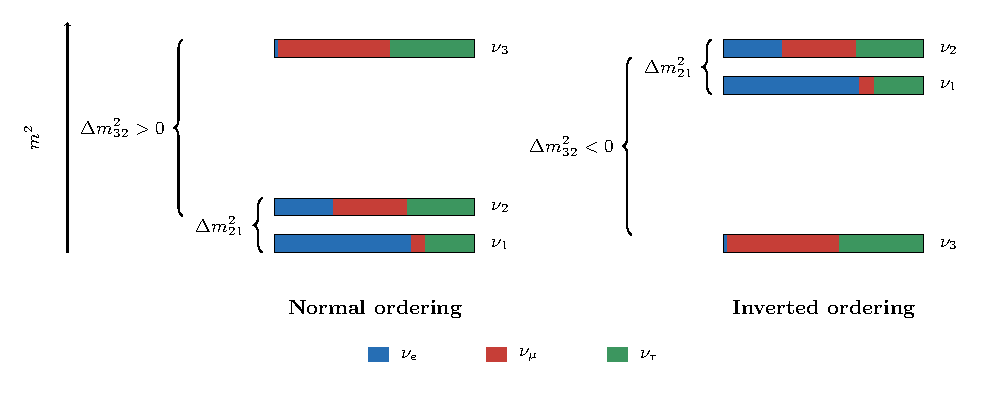
\includegraphics[width=0.72\textwidth]{mass_ordering.pdf}
    \caption{The two possible orderings of the neutrino mass states. The solar splitting
    $\dm{21}$ is known to be positive and is much smaller than the atmospheric splitting
    $|\dm{32}|$, which is drawn compressed here. Shading indicates the approximate flavour
    composition $|U_{\alpha j}|^{2}$ of each mass state.}
    \label{fig:mass-ordering}
\end{figure}

% Although the leading two-flavour term depends only on $|\dm{32}|$, the exact disappearance probability in Eq.~\hyperref[eq:pmumu-exact]{(\ref{eq:pmumu-exact})} contains both atmospheric frequencies, $\dm{31}$ and $\dm{32}$, separated by the known positive solar splitting.
% Their combination can be expressed as the effective splitting measured in $\numu$ disappearance~\cite{NunokawaParkeValle2008},
% \begin{equation}
%     \dm{\mu\mu} =
%     \sin^{2}\theta_{12}\dm{31}
%     + \cos^{2}\theta_{12}\dm{32}
%     + \cos\dcp\sin\theta_{13}\sin2\theta_{12}\tan\theta_{23}\dm{21}.
%     \label{eq:dm-mumu}
% \end{equation}
% The first disappearance minimum occurs at $E_{\rm dip}\simeq |\dm{\mu\mu}|L/2\pi$.
% Reversing the ordering changes how the positive solar-scale correction combines with the atmospheric splitting and therefore shifts the predicted location of this dip.
% The measured disappearance spectrum consequently provides sensitivity to the mass ordering through the dip position, rather than through the depth of the deficit.

\subsubsection*{The electron neutrino appearance probability}
The appearance channel contains and is therefore sensitive to parameters that disappearance cannot reach, and it is the origin of the degeneracies that complicate a joint fit.

To derive the $\nu_e$ appearance probability, it is helpful to start from the $\nu_\mu \rightarrow \nu_e$ transition amplitude, rather than Eq.~\hyperref[eq:three-flavour-general]{(\ref{eq:three-flavour-general})}.
As mentioned, a $\numu$ flavour state is a superposition of mass eigenstates, that each propagates with its own phase. For appearing $\nue$s, these are then projected onto the $\nue$ state when detected.
In analogy to Eq.~\hyperref[eq:amplitude]{(\ref{eq:amplitude})}, the appearance amplitude can be written as a coherent sum over the three mass eigenstates,

\begin{equation}
    A(\numu \to \nue)
    = \sum_{j=1}^{3} U_{e j}\,U_{\mu j}^{*}\,e^{-i\phi_j},
    \qquad
    \phi_j \simeq \frac{m_j^{2}L}{2E}.
    \label{eq:pmue-amplitude-sum}
\end{equation}

Since $\nu_1$ and $\nu_2$ are separated by a small $\dm21$, with $\nu_3$ separated by a $\dm \approx 10^{-5}$, it can be useful to the three terms into two amplitudes. An atmospheric amplitude (one most closely associated with the fast oscillations of the term arising from the $j=3$ term) and a so called solar amplitude (the slow development of the solar phase between $\nu_1$ and $\nu_2$ allows us group these together).              
By inserting the PMNS matrix elements of Eq.~\hyperref[eq:pmns-elements]{(\ref{eq:pmns-elements})}, the atmospheric amplitude, dominated by the $\nu_3$ term can be written as:
\begin{equation}
    A_{\rm atm} \sim U_{e3}U_{\mu 3}^{*}\,e^{-i\phi_3}
    \sim s_{13}s_{23}\,e^{-i(\phi_3+\dcp)},
    \label{eq:atm-amplitude}
\end{equation}
where $c_{13} \approx 1$.
The $\nu_1$ and $\nu_2$ terms are taken and combined into the solar amplitude:
\begin{equation}
    A_{\rm sol} \sim U_{e1}U_{\mu 1}^{*}\,e^{-i\phi_1} + U_{e2}U_{\mu 2}^{*}\,e^{-i\phi_2}.
    \label{eq:sol-amplitude}
\end{equation}

The probability is the squared magnitude of the total amplitude, therefore,
\begin{equation}
    P(\numu\to\nue) = |A_{\rm atm} + A_{\rm sol}|^{2}
    = |A_{\rm atm}|^{2} + |A_{\rm sol}|^{2} + 2\,\mathrm{Re}(A_{\rm atm}^{*}A_{\rm sol}).
    \label{eq:pmue-amplitude}
\end{equation}
After expanding in the small quantities $s_{13}$ and $\Delta_{21}$, the appearance probability takes the form given by~\cite{NunokawaParkeValle2008,Cervera2000}:
\begin{equation}
    P(\numu \to \nue) \simeq P_{\rm atm} + P_{\rm sol}
    + 2\sqrt{P_{\rm atm}P_{\rm sol}}\,\cos\!\left(\Delta_{32} + \dcp\right),
    \label{eq:pmue-red}
\end{equation}
with
\begin{equation}
    P_{\rm atm} = \sin^{2}\theta_{23}\sin^{2}2\theta_{13}\sin^{2}\Delta_{31},
    \qquad
    P_{\rm sol} = \cos^{2}\theta_{23}\cos^{2}\theta_{13}\sin^{2}2\theta_{12}\sin^{2}\Delta_{21}.
    \label{eq:patm-psol-red}
\end{equation}
The interference term depends on the relative phase of the two amplitudes, which contains both the propagation phase and $\dcp$; it is the only term in Eq.~\hyperref[eq:pmue-red]{(\ref{eq:pmue-red})} that depends on $\dcp$. Vacuum appearance measurements are therefore sensitive to CP violation, in contrast to the disappearance channel.
The antineutrino takes the complex conjugate of the matrix elements, flipping the sign of $\dcp$ in Eq.~\hyperref[eq:pmue-red]{(\ref{eq:pmue-red})}. This interference term therefore takes a different value for neutrinos compared to antineutrinos, both vanishing when CP is conserved.

Furthermore, in addition, $\theta_{23}$ enters the leading order $P_{atm}$ term via $\sin^2\theta_{23}$, in contrast to $\sin^22\theta_{23}$ in the disappearance case. The symmetry about $\pi /4$ is no longer present, which suggests that vacuum appearance data can, unlike $\numu$ disappearance can resolve the octant of $\theta_{23}$. These are vacuum expressions, however. The effect of neutrinos travelling through matter is particularly important for the appearance channel. The following subsection touches on how neutrino propagation through matter changes the oscillation probability.










% ============================================================================
\subsection{Matter Effects}
\label{sec:matter}
So far, the probability expressions, statements and derivations made above have assumed neutrino propagation in vacuum. 
In practice however, neutrinos propagate through matter, whether through the Earth, or through the Sun. As they travel, they undergo coherent forward elastic scattering from the matter particles. 
Since this is elastic scattering, their momenta are unchanged. 
However, matter consists almost entirely of electrons, rather than $\mu$ or $\tau$ leptons. Therefore, $\nue$s have access to these additional charged-current scattering interactions. As they propagate, they accumulate an additional relative phase, which is observable \cite{Wolfenstein1978,Mikheyev1985,Mikola2023}.
Figure~\ref{fig:matter-scattering} shows these two additional scattering processes for $\nue$s (left and centre). The right diagram shows the neutral-current process, which has equal probability for all three flavours.

In the case of $\nue$, this manifests as an additional potential energy term that enters the Hamiltonian, given by:

\begin{equation}
    V_{\rm CC} = \pm\sqrt{2}\,G_F N_e ,
    \label{eq:matter-potentials}
\end{equation}
with $N_e$ being the electron number density and $G_F$ the Fermi constant. The positive sign is for neutrinos and the negative sign is for antineutrinos. 
The NC phase shift is a global one, as it applies to all three flavours equally, so no relative phase accumulates and the oscillation probability is unaffected.
Neutral-current scattering gives every flavour the same shift, so it does not change their relative phases and therefore does not change the oscillation probability.

The simpler case of two-flavours is considered to understand the effect of $V_{\rm CC}$. In the mass basis, the vacuum Hamiltonian is diagonal. Using the two-flavour mixing matrix $U_2$ introduced in
Eq.~\hyperref[eq:two-flavour-mixing-matrix]{(\ref{eq:two-flavour-mixing-matrix})},
the Hamiltonian can be rotated to the flavour basis, and is given by:
\begin{equation}
    H_f^{(2)} =
    \frac{1}{2E}\,U_2
    \begin{pmatrix} 0 & 0 \\ 0 & \Delta m^2 \end{pmatrix}
    U_2^{\dagger}
    +
    \begin{pmatrix} V_{\rm CC} & 0 \\ 0 & 0 \end{pmatrix}.
    \label{eq:matter-hamiltonian}
\end{equation}

Considering the vacuum case, the Hamilatonian is diagonal in the mass basis. Each mass state therefore picks up its own phase as it propagates. In contrast, considering the matter case, as shown above, the Hamiltonian contains an additional potential term that is now diagonal in the flavour basis, not the mass basis. This potential therefore only affects the $\nue$ energy level, leaving the other flavours unaffected. 
With the addition of this potential, the independent vacuum mass states are replaced by new independent matter eigenstates.

This matter Hamiltonian can be diagonalised, defining a new effective mixing angle ($\theta_M$) and mass splitting ($\Delta m_M^2$). In two flavours, the familiar appearance probability expression can be written in terms of these new parameters as:
\begin{equation}
    P_M(\numu\to\nue) = \sin^2(2\theta_M) \sin^2\left(\frac{\Delta m_M^2L}{4E}\right).
    \label{eq:two-flavour-matter-probability}
\end{equation}
It can be shown that~\cite{Booth2021}
\begin{equation}
    \sin(2\theta_M) \equiv \frac{\sin(2\theta)}{A_M},
    \qquad
    \Delta m_M^2 \equiv \Delta m^2 A_M,
    \label{eq:matter-effective-params}
\end{equation}
where the factor $A_M$ rescales the vacuum mixing angle and mass splitting into their effective equivalents in matter,
\begin{equation}
    A_M = \sqrt{\left(\cos(2\theta)\mp\frac{2EV_{\rm CC}}{\Delta m^2}\right)^2 + \sin^2(2\theta)}.
    \label{eq:matter-factor}
\end{equation}
The effect of neutrinos versus antineutrinos on the oscillation probability is clear to see through the $\mp$ sign in Eq.~\hyperref[eq:matter-factor]{(\ref{eq:matter-factor})}, where minus sign for neutrinos is flipped for antineutrinos.

At NOvA, the matter effect enhances the appearance probability for the normal ordering and suppresses it for the inverted ordering hypothesis. The effect is also reversed in the antineutrino case, due to the sign flip as described above. 

\begin{figure}[htbp]
    \centering
    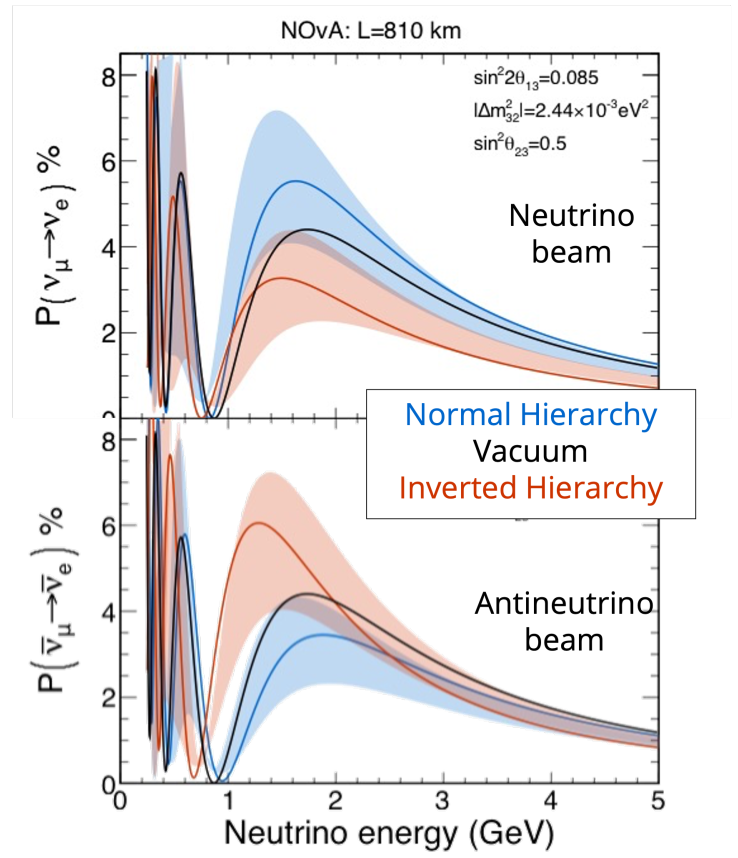
\includegraphics[width=0.68\textwidth]{nova_matter_probability.png}
    \caption{The $\numu\to\nue$ (upper) and $\numubar\to\nuebar$ (lower)
    appearance probabilities at NOvA.  The black curve is the vacuum
    probability; blue and orange show normal and inverted ordering in matter
    at $\dcp=0$, with the bands spanning the allowed values of $\dcp$.
    Reproduced from NOvA internal note 21764~\cite{CatanoMur2017}, as used in
    Figure~1.8 of Ref.~\cite{Mikola2023}.}
    \label{fig:nova-matter-probability}
\end{figure}

Considering the first oscillation maximum of Figure~\ref{fig:nova-matter-probability}, it is clear that with the inclusion of matter effects, the appearance probability is enhanced for the normal ordering hypothesis and it is suppresed for the inverted ordering case. The shaded regions show that varying the value of $\dcp$ can also shift the appearance probability in both directions. As a consequence, a normal ordering hypothesis with a $\dcp$ value that lowers the appearance probability can be such that it is consistent with an inverted ordering hypothesis with a different $\dcp$ value enhances the apeparance probability. This leads to a degeneracy between the mass ordering and $\dcp$. Measuring an appearance probability near the vacuum curve or the shaded overlap region does not allow for either the mass ordering  The addition of antineutrino appearance data would help to resolve this degeneracy. This is due to both the matter potential, $V_{\rm CC}$, and the CP violating term, $\dcp$ changing sign relative to the neutrino case. Combinations of mass ordering and $\dcp$ values that give the same neutrino appearance probability will give different probabilities for the antineutrino case.

The combination of neutrino and antineutrino appearance data helps to disentangle this degeneracy, but with current low statistics, the mass ordering and $\dcp$ questions remain open. 
Section~\ref{sec:landscape} touches on some experiments that contrain the parameters belonging to each sector.  
\clearpage



% % !TEX root = ../main.tex
\section{Spectrum and Sensitivity}
\label{sec:spectrum}
\label{sec:sensitivity}

% Combines the pedagogical ``what features appear in the spectrum'' discussion with
% the measurement-strategy / sensitivity arguments. Target ~7--8 pp total.

\subsection{Probability versus $L/E$}
% Global $P(L/E)$ --- fast atmospheric wiggle + slow solar envelope --- one
% paragraph and one figure.

\subsection{The NOvA Oscillation Window}
% Zoom to NOvA ($L=810$\,km, $E\sim 1$--$3$\,GeV): a narrow $L/E$ slice spanning
% one atmospheric oscillation cycle, not multiple wiggles. Physics motivation for
% this baseline and energy: sits at the oscillation maximum for $\Delta m^{2}_{32}$
% and gives a matter effect large enough to help break the ordering--$\delta_{\rm CP}$
% degeneracy. Numbers only; no hardware.

\subsection{The Disappearance Spectrum}
% FD disappearance: single broad dip --- position fixes $\Delta m^{2}_{32}$,
% depth fixes $\sin^{2}(2\theta_{23})$. Why the dip region ($L/E\sim L_{\rm osc}/2$)
% gives the sharpest $\Delta m^{2}_{32}$ handle.

\subsection{The Appearance Spectrum}
% FD appearance: single broad peak --- rate carries $\theta_{13}\times\delta_{\rm CP}$
% interference and (via matter) mass ordering; shape carries less information.
% $\nu$ vs $\bar\nu$ running.
% Appearance vs disappearance probe orthogonal parameter combinations.
% $\delta_{\rm CP}$ appears only in appearance (interference term);
% $\nu_e$/$\bar\nu_e$ rate difference is the primary CP handle.
% Small derivation of matter-modified $P(\nu_\mu\to\nu_e)$ (Nunokawa--Parke--Valle
% expansion; not a full three-eigenvalue diagonalisation). Consequence:
% $\nu$/$\bar\nu$ asymmetry combines matter + $\delta_{\rm CP}$ degenerately;
% a long baseline separates them because matter scales differently with $E$.

% !TEX root = ../main.tex
\section{Experimental Landscape}
\label{sec:landscape}

% Spine (2026-08-09 grilling; next-gen/close 2026-08-27): solar/reactor -> LBL
% (NOvA/T2K; inline T2K--NOvA joint + JUNO--LBL |dm^2| ordering hook; brief
% IceCube) -> DUNE-weighted next-generation (DUNE Phase I/II + exposure-indexed
% reach; Hyper-K short; complementarity) -> NuFIT 6.1 table + pointer
% opens / meantime NOvA disappearance handoff. Intro: provenance claim; body:
% programme sectors. Citation convention: page numbers refer to the arXiv
% version named in each bib entry, not to journal pagination. Sources cited by
% table or figure number use pagination-independent identifiers. See the header
% comment in main.bib. See ADR-0003.

The physics describing neutrino oscillations was set out in the previous section. This
included the three-flavour oscillation framework, which helped to introduce 
the PMNS mixing matrix and the six oscillation parameters that govern flavour change in vacuum.
Matter effects were also introduced and shown to modify the oscillation probabilities. 
This section turns to the current status of our knowledge of these parameters and the 
experiments that constrain them, past, current and future. Many experiments world wide, probing 
the different sectors, which are definted by their distinct $L/E$ ratios and the flavours they can tag,
are each sensitive to their own set of oscillation parameters. This section outlines the
experimental programmes that measure the parameters of each sector, and subsequently 
summarising the global picture. Whilst the discussion will show the current understanding 
which includes precise measurements, three main open questions still remain. Namely, the mass ordering, 
the octant of $\theta_{23}$ and the value of $\dcp$~\cite{NuFIT60,NuFIT61}. Future next genration experiments seek to 
address these open questions, and will also be discussed.
 

% ============================================================
\subsection{Solar and Reactor Measurements}
\label{sec:landscape-solar-reactor}



\paragraph{The solar sector.}
As touched on in Sec.~\ref{sec:history-anomalies}, the solar deficit was first observed
by the Homestake experiment, providing a first indication of neutrino oscillations.
Super-Kamiokande and SNO then provided further compelling experimental evidence for such
flavour change~\cite{Fukuda2001,Ahmad2002}. However, it was only a year later, in 2003, when
the Kamioka Liquid Scintillator Antineutrino Detector (KamLAND) first provided initial
constraints on the solar parameter pair $(\theta_{12},\dm{21})$~\cite{KamLAND2003}. 
Each of these experiments probe the solar sector; with neutrinos produced in nuclear reactions 
in the Sun being the primary source for Super-Kamiokande and SNO. And reactor neutrinos being the 
source for KamLAND. Super-Kamiokande measures neutrinos via $\nu$--electron elastic scattering in 
a large water Cherenkov detector, whilst SNO uses a heavy-water Cherenkov detector to allow for NC, 
CC and elastic scattering interactions to be separately tagged. KamLAND instead measures the disappearance
of reactor $\nuebar$ with a liquid-scintillator detector at a flux weighted average distance of 
$180$\,km~\cite{KamLAND2003}. Super-Kamiokande and SNO therefore probe the solar parameters 
with matter effects via the traversing of the neutrinos through the falling electron density in 
the Sun's core, whilst KamLAND's provides a complementary determination of these parameters 
without such effects. Solar matter effects helped fix the sign of $\dm{21}$ and resolve the octant
of $\theta_{12}$, which reactor experiments like KamLAND could not do alone. $\dm{21}$ was therefore
found to be a positive quantity. Subsequently, KamLAND was able to confirm the values of these
parameters with higher precision in the vacuum case~\cite{KamLAND2013}.





\paragraph{JUNO and the solar sector today.}
\label{sec:landscape-juno}
With the start of data taking in 2025, the first results from the Jiangmen 
Underground Neutrino Observatory (JUNO) have substantially improved the 
solar picture. JUNO is a $20$\,kt liquid-scintillator detector located such that is is 
equidistant to all reactor cores from the Yangjiang and Taishan reactor complexes~\cite{JUNO2026}. 
The reactor $\nuebar$ are detected via inverse beta decay and this baseline was chosen
such that the $L/E$ sits close to the first disappearance minimum.
Figure~\ref{fig:juno-pee-baseline} shows the slow solar and fast atmospheric oscillations in
the $\nuebar$ survival probability as a function of a baseline, considering a fixed 
$4$\,MeV recator neutrino energy. JUNO, DayaBay and KamLAND are placed on this plot for 
comparison.

\begin{figure}[tb]
    \centering
    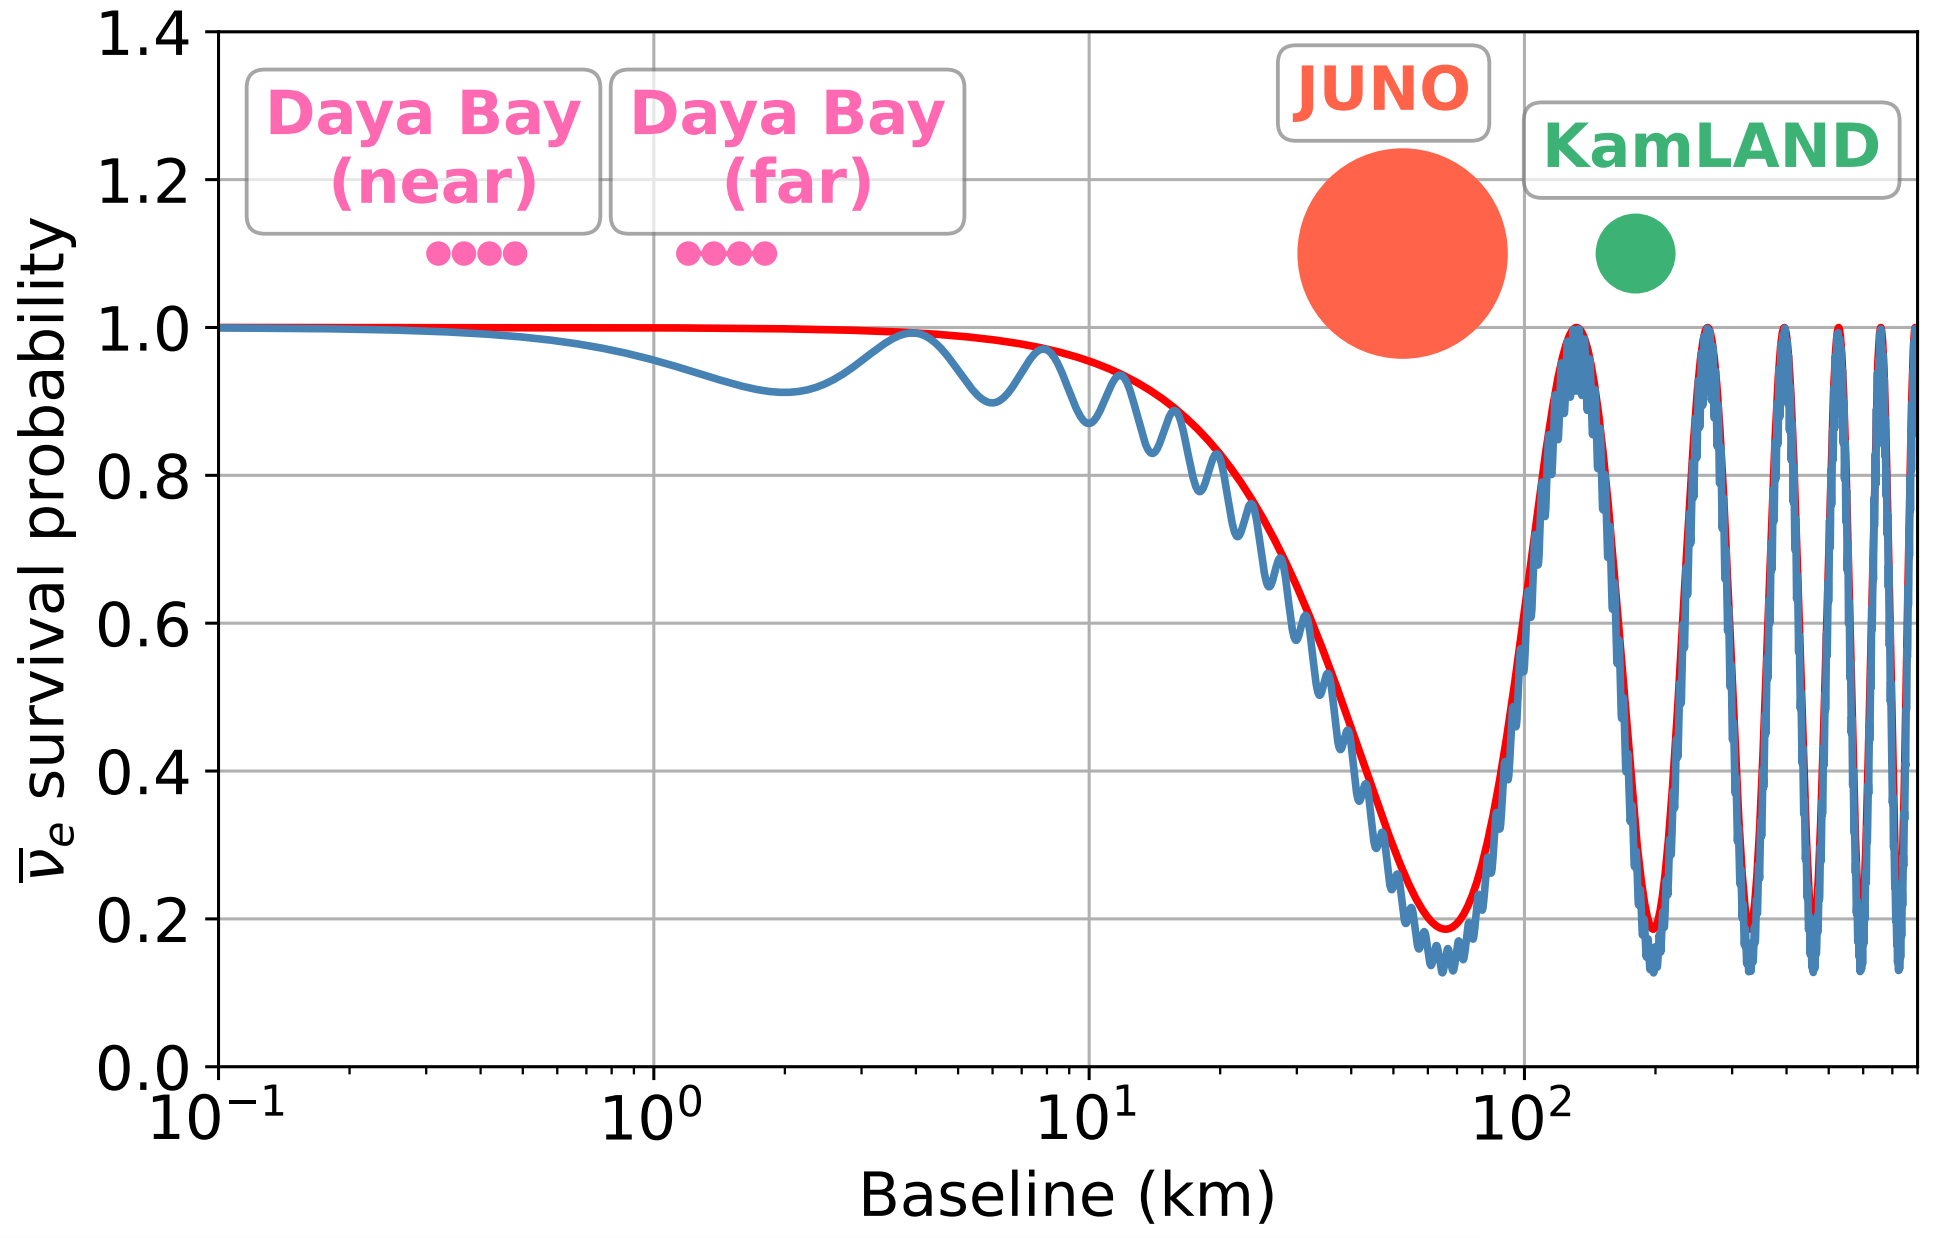
\includegraphics[width=0.85\textwidth]{slow_fast_nue_osc_2.png}
    \caption{$\nuebar$ survival probability as a function of baseline at fixed $4$\,MeV reactor 
    energy. The red curve indicates the slow oscillations driven by the solar splitting, $\dm{21}$, 
    while the blue curve shows the full survival probability, which includes the fast atmospheric 
    oscillations due to $\dm{31}$. The JUNO baseline of $52.5$\,km sits near the first solar disappearance
    minimum; Daya Bay (near/far) and KamLAND are shown for comparison. Reproduced from the
    JUNO Collaboration~\citep[Fig.~5]{JUNO2026}.}
    \label{fig:juno-pee-baseline}
\end{figure}
After just $59.1$\,days of data collected, JUNO's first results were relased, reporting a
simultaneous high-precision determination of both solar oscillation parameters, $\sin^{2}\theta_{12}$ 
and $\dm{21}$~\cite{JUNO2026}:
\begin{equation}
    \sin^{2}\theta_{12} = 0.3092 \pm 0.0087,
    \qquad
    \dm{21} = (7.50 \pm 0.12)\times 10^{-5}~\text{eV}^{2}.
    \label{eq:juno-solar}
\end{equation}
This result represents a substancial improvement on the precision of the previous combined 
measurements by a factor of 1.6 when considering the normal mass ordering scenario.
Figure~\ref{fig:juno-solar} shows JUNO's $\dm21$ vs $/sin^2 \theta_{12}$ confidence intervals alongside 
results from the previously mentioned experiments. Comparing the error bars for each result shows
that a reactor measurement now leads the measurement of the solar pair of parameters.
However, results from solar data are still very important for the improvement in the determination
of the sign of $\dm{21}$ and the octant of $\theta_{12}$ via the matter effects from neutrino propagation 
in the Sun. 
\begin{figure}[tb]
    \centering
    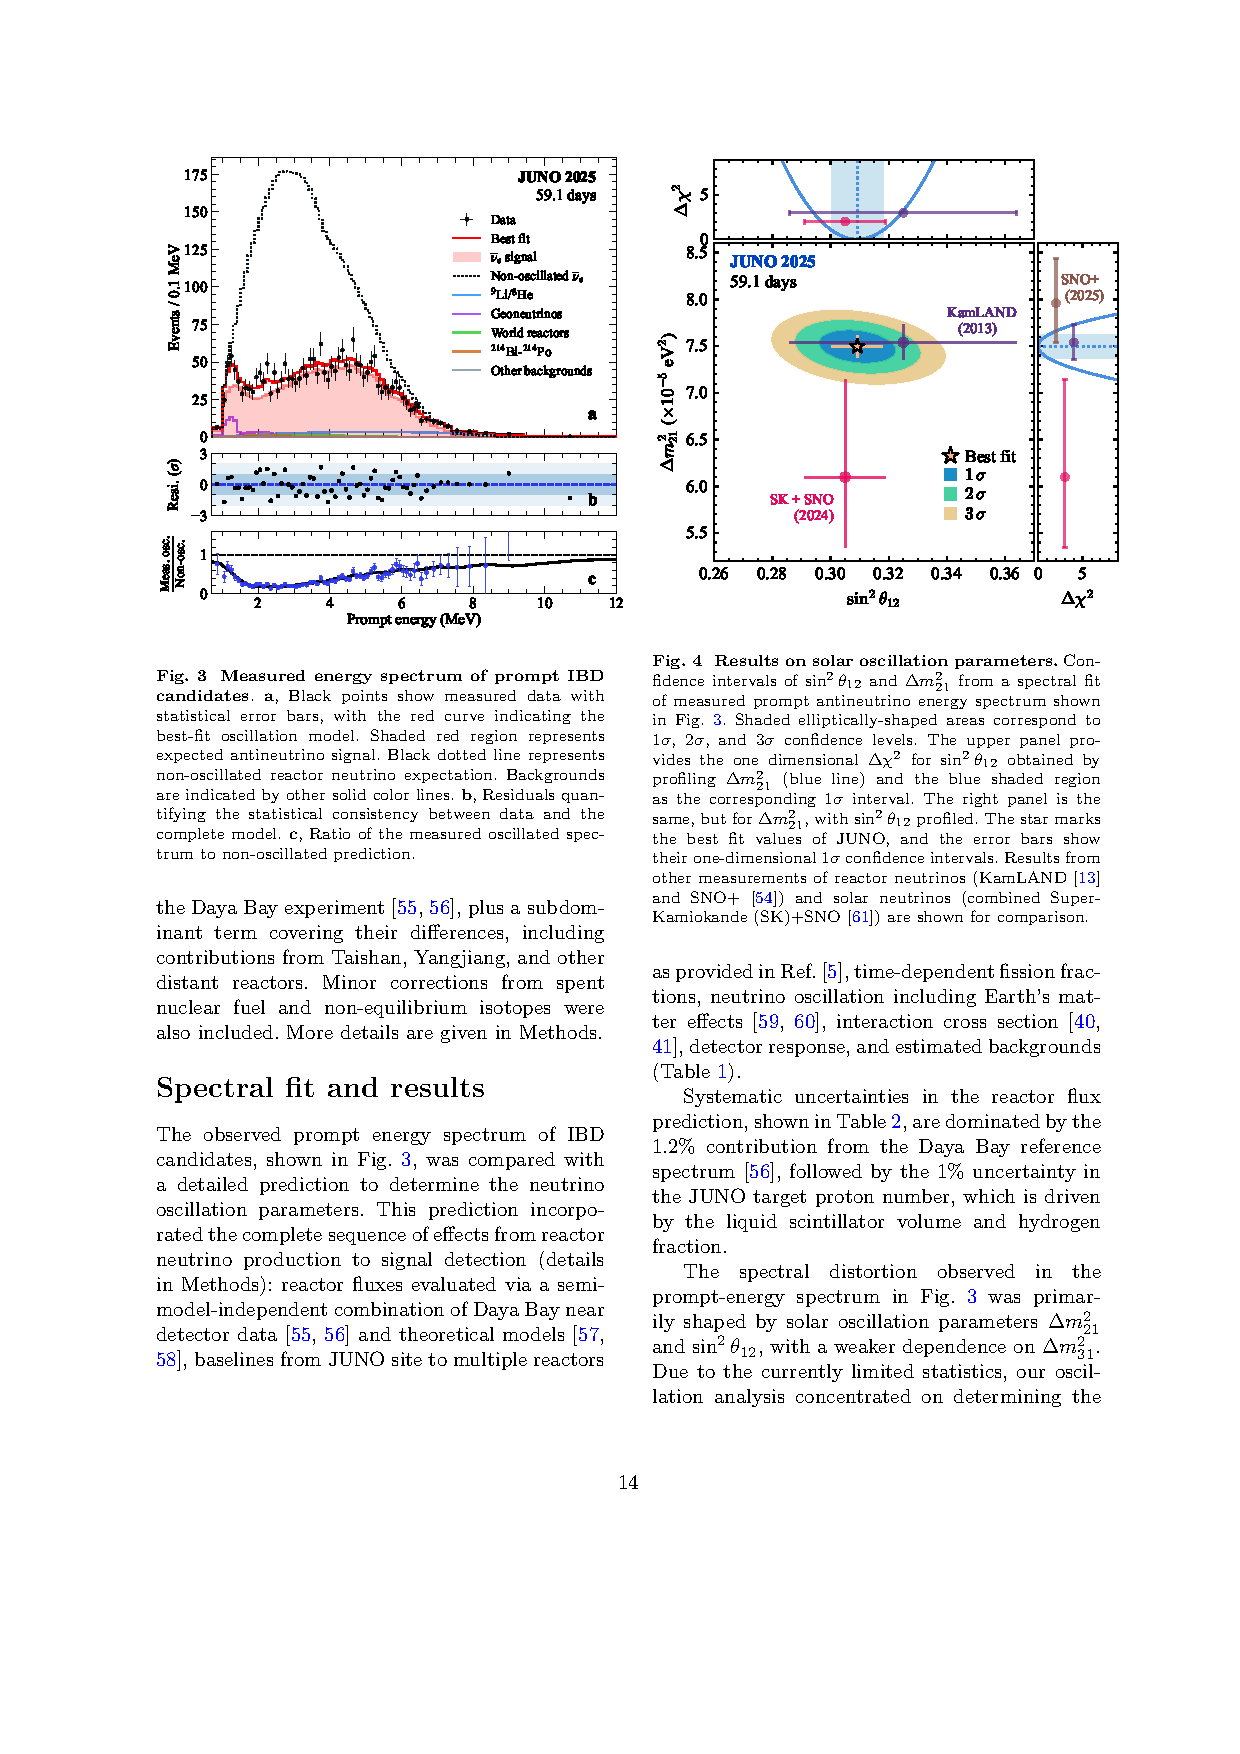
\includegraphics[trim=302bp 542bp 7bp 64bp,clip,width=0.70\textwidth]{juno_solar_src.pdf}
    \caption{Confidence intervals on $\sin^{2}\theta_{12}$ and $\dm{21}$ from the first
    JUNO data set, with the KamLAND and combined Super-Kamiokande\,+\,SNO determinations
    shown for comparison. The side panels give the one-dimensional $\Delta\chi^{2}$
    profiles. Reproduced from the JUNO Collaboration~\citep[Fig.~4, p.~14]{JUNO2026}.}
    \label{fig:juno-solar}
\end{figure}
It's useful to note that for JUNO's first results, the $\theta_{13}$ and $\dm{31}$ parameters are input 
as external constraints and are not fitted outputs. 
% The Daya Bay short-baseline reactor experiment, provides the leading $\theta_{13}$ measurement, which is what is used in JUNO's fit. 
JUNO's position along the blue curve of Figure~\ref{fig:juno-pee-baseline} is such that it can
also resolve these fast oscillations and hence measure the atmospheric mass splitting $|\dm{31}|$. 
This is a measurement JUNO has performed (\textcolor{red}{no arxiv for $\dm{31}$ result yet}).
Such measurements are also used as external constraints in Long Baseline (LBL) accelerator experiments, 
which will be discussed later.

Super-Kamiokande were the first to establish the parameters pertaining to the atmospheric sector, namely
$\theta_{23}$ and $\dm{32}$. This was achieved by using the zenith angle of atmospheric neutrino 
interactions to estimate their path lengths through the Earth, from down-going to up-going, thereby 
achieving different baselines. Today however, accelerator long-baseline experiments lead the precision 
on these parameters (Sec.~\ref{sec:landscape-lbl}). Since the leading order term in the appearance probability
goes as $P_{\rm atm}$~\hyperref[eq:patm-psol-red]{(\ref{eq:patm-psol-red})} and LBL experiments have weak 
$\theta_{31}$ sensitivity, like JUNO, external constraints on this parameter are essential.

Such a constraint comes from the short-baseline reactor experiment of Daya Bay, in China, which is located
between the Daya Bay and Ling Ao reactor complexes and measures $\nuebar$ disappearance.
At a baseline of $\approx 1.6 km$, the leading order $\dm{31}$ oscillations term sits near
the first disappearance minimum, with the depth of the dip isolating $\theta_{13}$. With two near 
detector halls to constrain the flux and $\nuebar$ spectrum and the far detector halls measuring the $\nuebar$ 
deficits\footnote{These are the two Daya Bay (near/far) markers in Fig.~\ref{fig:juno-pee-baseline}}, 
Daya Bay's result from its final dataset collected over $3158$ days \cite{DayaBay2023} leads the measurement 
for $\theta_{13}$:
\begin{equation}
    \sin^{2}2\theta_{13} = 0.0851 \pm 0.0024.
    \label{eq:dayabay-theta13}
\end{equation}

% Its importance for long-baseline physics is indirect but decisive. Because reactor
% $\nuebar$ disappearance has no $\dcp$ dependence and a negligible matter effect,
% Eq.~\eqref{eq:dayabay-theta13} can be imported into accelerator appearance fits as an
% external prior. Without it the $\nue$ appearance rate would be a function of two
% unknowns at once ($\theta_{13}$ and $\dcp$, entangled also with the mass ordering), and
% neither $\dcp$ nor the ordering could be cleanly extracted. This is why NOvA's
% three-flavour oscillation analyses, discussed in Sec.~\ref{sec:landscape-lbl}, are
% quoted both with and without the Daya Bay $\theta_{13}$ constraint applied.

% ============================================================
\subsection{Long-Baseline Accelerator Measurements}
\label{sec:landscape-lbl}

{\color{red}
\textit{Rough plan (grilling contract):}
\begin{itemize}
    \item NOvA: $\dm{32}$, $\theta_{23}$, weak ordering / $\dcp$ preference
    \item T2K: same parameters, shorter baseline (smaller matter effect)
    \item T2K--NOvA joint: brief \emph{inline} paragraph (no peer joint-fit subsection)
    \item JUNO--LBL $|\dm{3\ell}|$ ordering hook: conceptual only; quantitative later
    \item IceCube DeepCore: one or two sentences (wider programme; not next-gen)
\end{itemize}
}
Unlike solar or reactor experiments, long baseline accelerator experiments have far more control over both 
the baseline and the neutrino energy spectrum. They choose these such that the $L/E$ samples the first 
atmospheric oscillation maximum. The dip in the disappearance spectrum provides the principle 
$\dm{32}$ and $\sin^2(2\theta)$ sensitivity, while the appearance sample allows for the $\dcp$, the ordering and
the octant of $\theta_{23}$ to be inferred.




\paragraph{NOvA.}
The NOvA experiment, whose setup will be discussed in the next chapter, utilises a baseline of $810$\,km
and has an energy spectrum that peaks between the $1$--$3$\,GeV range, such that it sits near that first 
oscillation maximum.
NOvA's latest full 3-flavour oscillation result analyses its full ten-year data set, with an exposure of
$26.61\times10^{20}$ and $12.50\times10^{20}$ protons on target (POT) in neutrino and
antineutrino beam modes respectively. It fits the $\numu$, $\numubar$, $\nue$ and
$\nuebar$ samples simultaneously, the details of which will be discussed in a later chapter. 
NOvA boasts the most precise single experiment constraint on the atmospheric mass squared splitting 
$\dm{32} = 2.431^{+0.036}_{-0.034} (-2.479^{+0.036}_{-0.036})\times 10^{-3}~\text{eV}^{2}$
for the normal (inverted) mass ordering hypothesis~\citep[p.~1]{NOvA2025}.
In both ordering hypotheses, a value for $\sin^{2}\theta_{23} = 0.55^{+0.02}_{-0.02}$, which sits near the 
maximal mixing case, was measured. No significant preference for the octant of $\theta_{23}$ was found.
The normal ordering hypothesis is slightly favoured with a Bayes factor or 2.4 compared to the inverted ordering,
indicating that the NO is 2.4 times more probable than the IO~\citep[p.~1]{NOvA2025}. Applying Daya Bay's
$\theta_{13}$ measurement as a 1-dimensionsl external constraint increases the preference to $3.3$ and adding their
constraint on the atmospheric splitting further raises it to $6.6$. These Bayes Factors are not yet large enough
to consider the ordering resolved.

Figure~\ref{fig:nova-contour} shows the allowed region in the $\dm{32}$--$\sin^{2}\theta_{23}$ space for NOvA,
as well as other experiments, showing NOvA's best fit point, which lies in the region favoured by the normal
ordering hypothesis. The summarised results above can be seen from this plot. The width of NOvA's 
allowed $90 \%$ confidence interval in $\dm{32}$ is the most narrow of all other plotted experiments, reinforcing
its claim as the most precise measurement for this parameter. In contrast, the $90 \%$ confidence region sits 
almost symmetrically about the $\sin^{2}\theta_{23} = 0.5$ line, which indicates maximal mixing, and that the 
octant of $\theta_{23}$, as mentioned, is not well constrained.


\begin{figure}[tb]
    \centering
    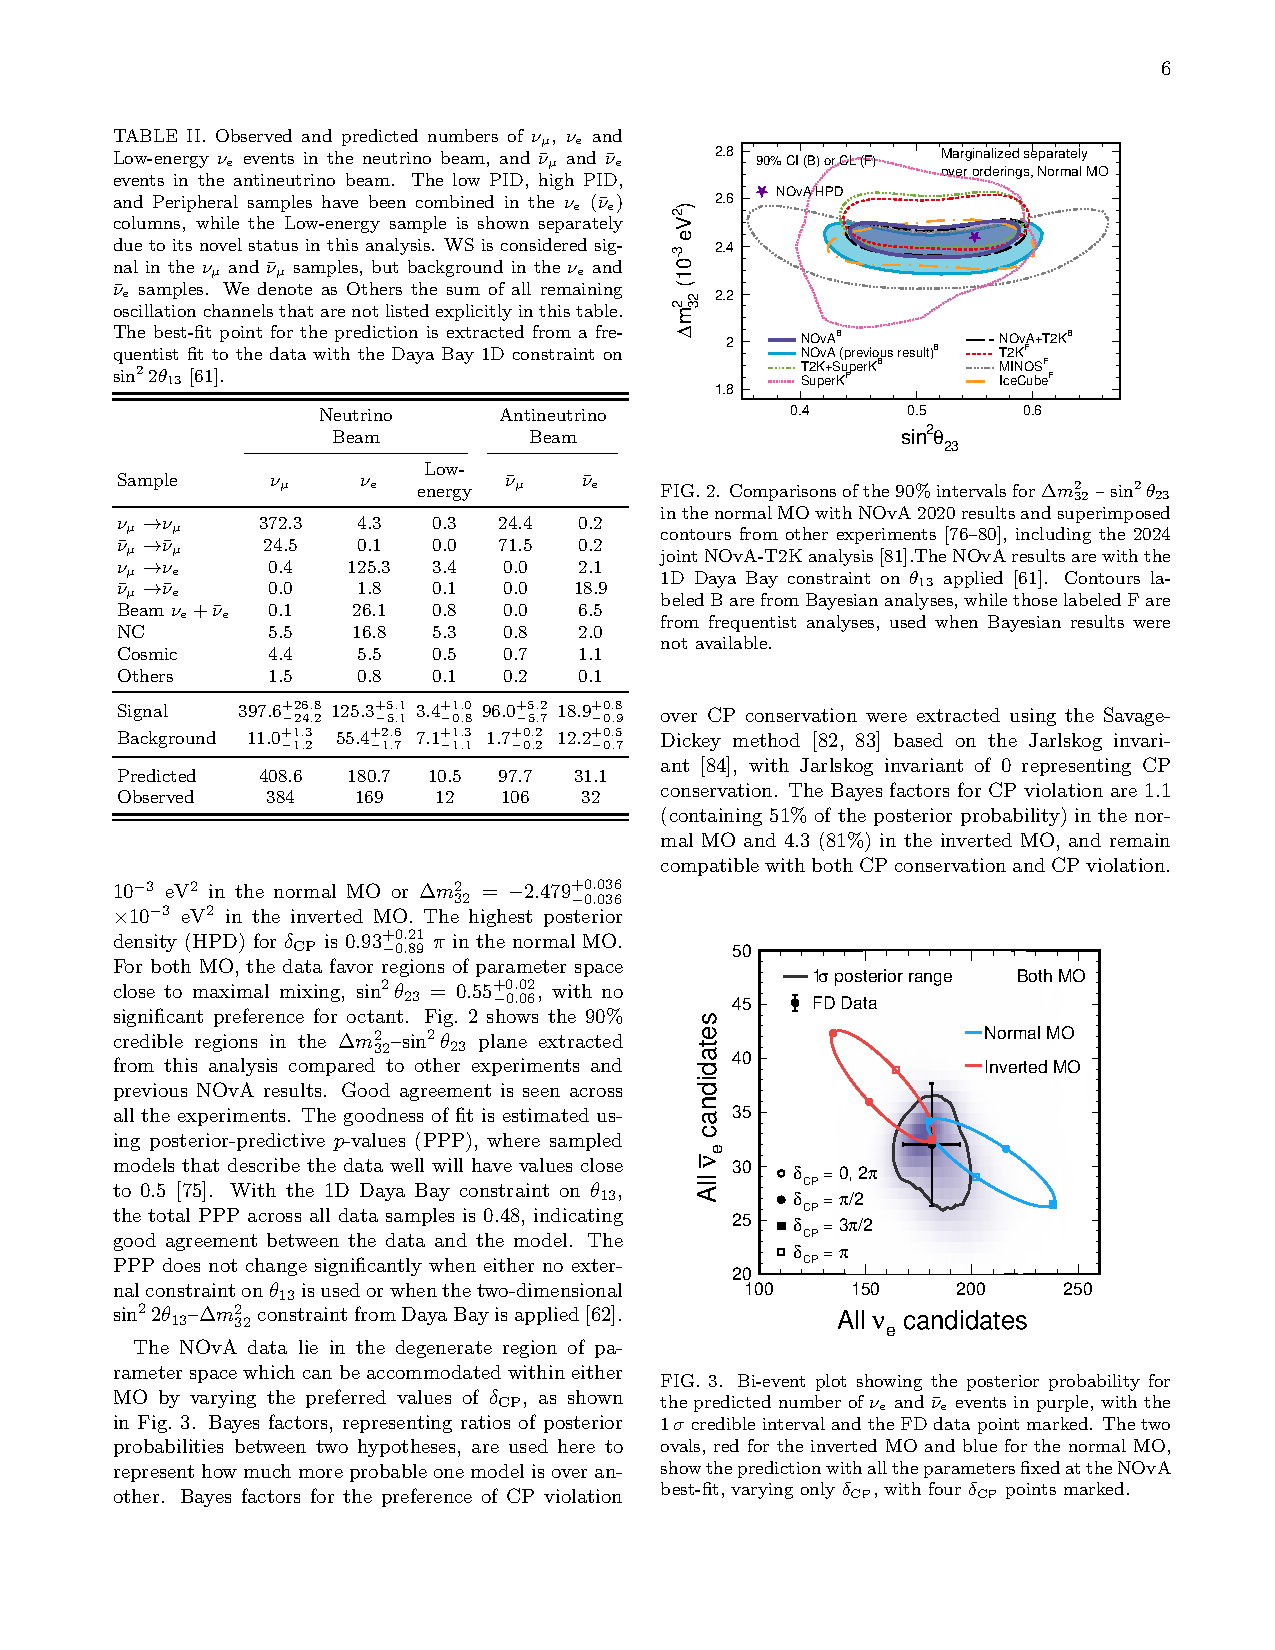
\includegraphics[trim=305bp 572bp 27bp 45bp,clip,width=0.66\textwidth]{nova_contour_src.pdf}
    \caption{NOvA's $90\%$ confidence interval in $\dm{32}$--$\sin^{2}\theta_{23}$ space. Plot compares NOvA and
    other experiments' results. NOvA's latest results region is shown with 1D Daya Bay $\theta_{13}$ external 
    constraint. Plot obtained from~\citep[Fig.~6]{NOvA2025}.}
    \label{fig:nova-contour}
\end{figure}

\paragraph{NOvA-T2K.}
The Tokai to Kamioka (T2K) experiment, measures the same parameters as NOvA, as it sits at a similar $L/E$.
T2K has a shorter baseline of $295$\,km and its energy spectrum peaks lower at around $0.6$\,GeV.
Both experiments sit near the first disappearance dip and as a result are broadly consistent in their 
disappearance measurements as can be seen in Figure~\ref{fig:nova-contour}.
Since NOvA's baseline is around $2.7\times$ larger than T2K's, NOvA's neutrinos pass through more of the Earth. The 
appearance channel for NOvA therefore sees an enhanced matter effect. As a consequence, the ordering--$\dcp$ 
degeneracy introduced in Section~\ref{sec:matter} manifests differently in both experiments. The bi-event plot
of Figure~\ref{fig:bievent} shows this more concretely. This plot shows the expected number of $\nuebar$ against $\nue$ 
appearance candidate events at NOvA (a) and T2K's (b) far detectors. By varying the value of $\dcp$ through a full 
period, from $-\pi$ to $\pi$, the predicted number of events traces out an ellipse in this space, with each ordering tracing 
out its own ellipse. The degeneracy explained in Section~\ref{sec:matter}, is clearly visible in the NOvA panel (a), that is, 
the appearance rate for the normal ordering hypothesis with $\dcp\simeq+\pi/2$ yields an almost identical rate to the 
inverted ordering hypothesis with $\dcp\simeq-\pi/2$. For these two hypotheses, the degeneracy occurs due to the matter term 
and the CP term cancelling, resulting in an almost identical appearance rate. With T2K's smaller matter effect, the ordering
sensitivity is weakened, which can be seen by the ellipses overlapping much more than in NOvA. This additional overlap means
that for maximal CP violation, the degeneracy is lifted slightly; the same $\dcp$ values coincide more closely in both 
orderings. For CP-conserving points, the opposite is true; the degeneracy between different CP-conserving values and the 
ordering is still present.

\begin{figure}[tb]
    \centering
    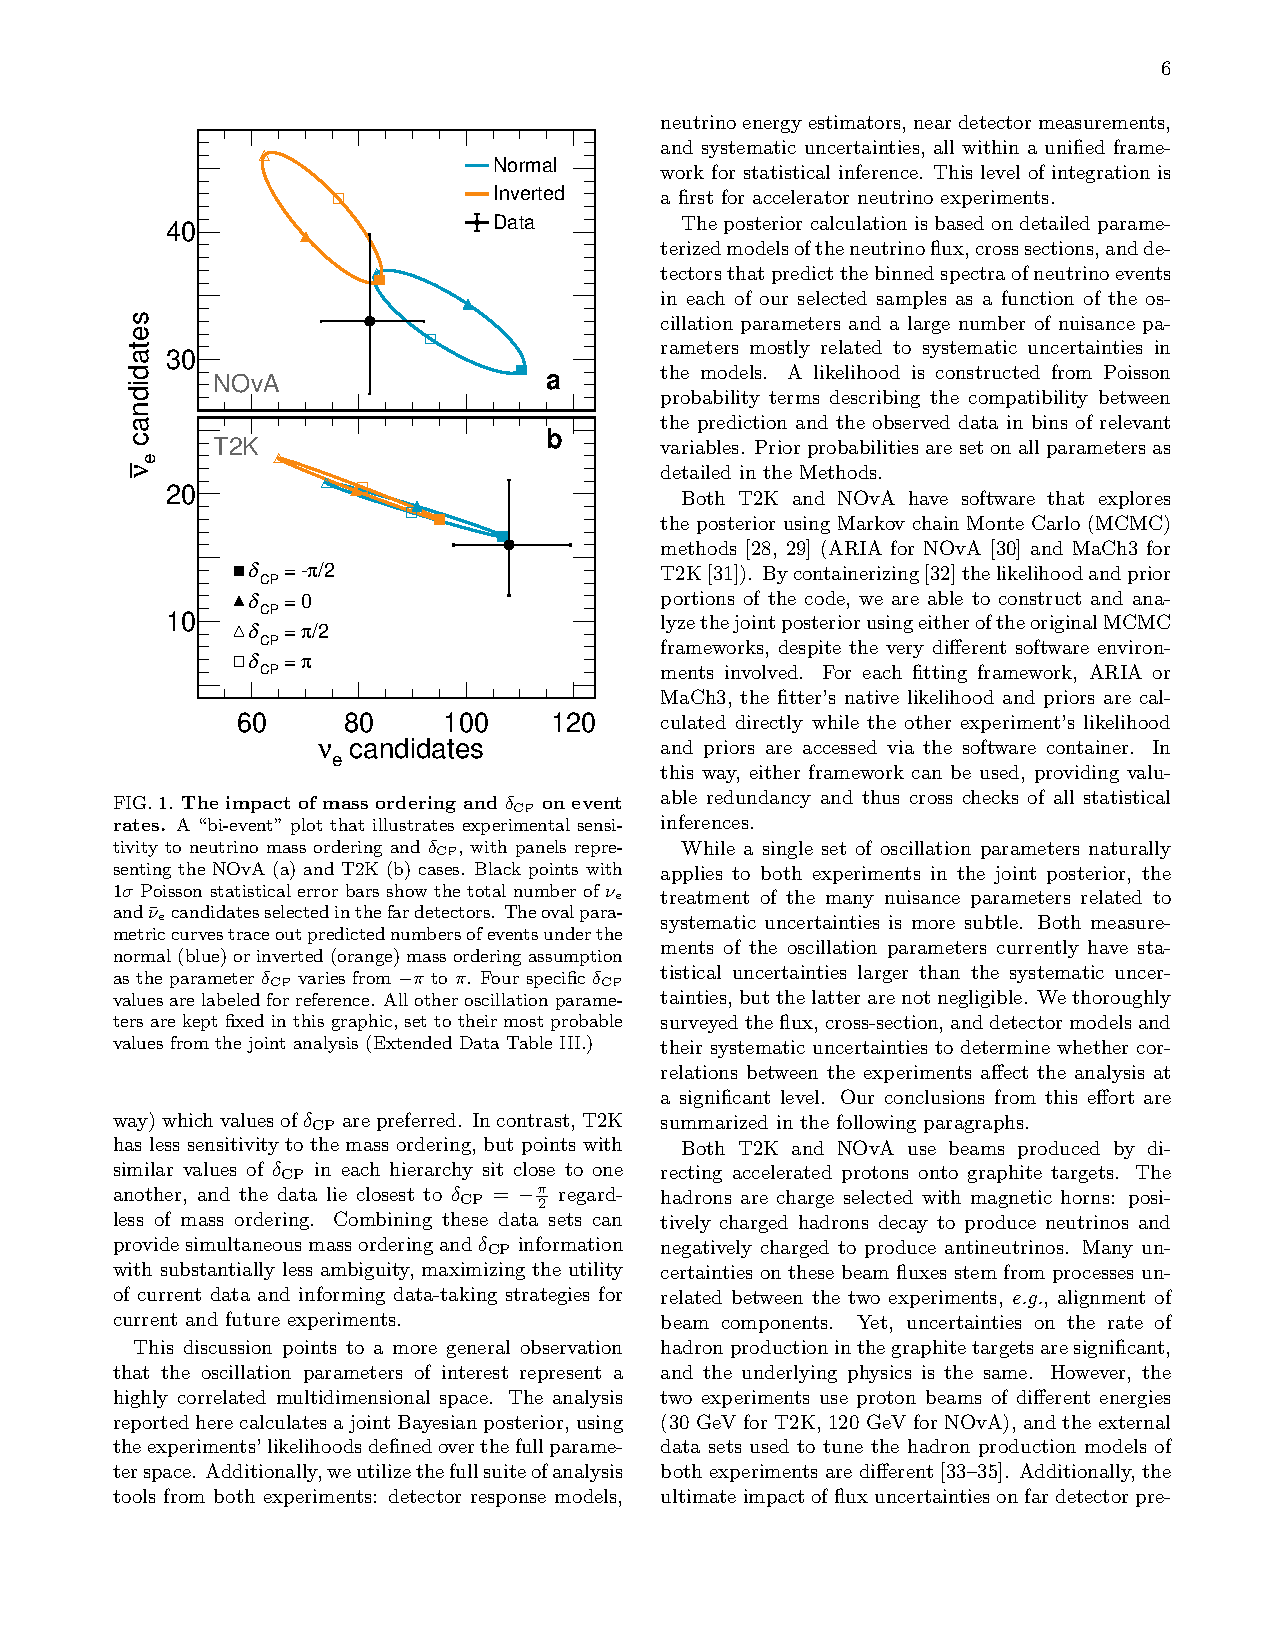
\includegraphics[trim=35bp 424bp 322bp 45bp,clip,width=0.48\textwidth]{novat2k_bievent_src.pdf}
    \caption{``Bi-event'' plot, which shows the predicted number of $\nue$ vs $\nuebar$ appearance
    candidate events for NOvA (a) and T2K (b). Varying $\dcp$ through its full range traces an ellipse,
    with four reference values of $\dcp$ marked, with one ellipse for the normal (blue), and one
    for the inverted (orange) orderings. Taken from the T2K and NOvA Collaborations~\citep[Fig.~1, p.~6]{T2KNOvA2025}.}
    \label{fig:bievent}
\end{figure}

Comparing the data points for both experiments, NOvA's point is closest to the overlap of the ellipses, occupying the most 
degenerate region, whereas T2K's is placed at the tip of the normal ordering ellipse corresponding to $\dcp\simeq-\pi/2$ in 
either ordering. Due to the pulling apart of the ellipses, NOvA is more sensitive to the ordering, whereas T2K's overlap makes
its $\dcp$ sensitivity stronger. For this reason, the joint analysis of the two experiments combines the appearance samples.


This first joint analysis yielded a value for $\dm{32} = 2.43^{+0.04}_{-0.03}(-2.48^{+0.03}_{-0.04})\times10^{-3}$\,eV$^{2}$ in 
the normal (inverted)ordering, with a $3\sigma$ interval on $\dcp$ of $[-1.38\pi,\,0.30\pi]$ in the normal ordering, narrowing 
to $[-0.92\pi,\,-0.04\pi]$ when assuming the inverted ordering ~\citep[p.~5]{T2KNOvA2025}. The joint collaboration performed a 
joint Bayesian posterior fit over a shared set of oscillation parameters. The fit showed no significant preference for either 
ordering. However, when the inverted ordering hypothesis is assumed, the fit excludes a substantial fraction of $\dcp$ space, 
and favours maximal CP violation with $\dcp\simeq-\pi/2$~\citep[Fig.~3, p.~9]{T2KNOvA2025}.


\paragraph{Reactor--accelerator complementarity.}
The determination of the atmospheric mass squared splitting parameter $\dm{3\ell}$ by reactor and long baseline
accelerator experiments are complementary in that their measurements should agree under the correct mass
ordering. Reactor $\nuebar$ disappearance experiments are sensitive to $|\dm{31}|$, whereas long-baseline $\numu$
disappearance measures $\dm{32}$. These two parameters, arising as frequencies in the oscillation probability, differ 
by the known solar splitting $\dm{21}$. Therefore, the two types of experiments should agree after subtracting the solar splitting
from $\dm{31}$ under the correct mass ordering hypothesis. A reactor measurement of $\dm{31}$ can therefore be used to help with 
the mass ordering determination in NOvA, an idea that will be fleshed out in a later chapter. As a results, as reactor experiments 
like JUNO matures and becomes more precise, NOvA will be able to improve its ordering preference~\cite{NOvAJUNO2026}.

% ============================================================
\subsection{Next-Generation Experiments}
\label{sec:landscape-nextgen}

\paragraph{DUNE.}
The Deep Underground Neutrino Experiment (DUNE) will send a wide-band neutrino beam $1300$\,km from Fermilab to
a far detector complex consisting of up to four liquid-argon time-projection chambers located at the Sanford
Underground Research Facility, with a movable near detector (DUNE-PRISM) on the Fermilab site~\cite{DUNE2025Science}. Matter effects are enhanced due to the much longer baseline
when compared to NOvA and T2K. DUNE's bi-event plot would show the ellipses no longer overlapping, meaning that no pair
of $\dcp$ values would coincide in both orderings. The separation of the ellipses indicates DUNE's highly enhanced
ordering sensitivity. In contrast, DUNE's $\dcp$ sensitivity cannot be enhanced enough by matter effects alone.
Even after the ellipses have been fuly separated thanks to increased matter effects, a single data point, lying on an ellipse 
will still have some degeneracy (in $\dcp$) caused by a change in $\theta_{23}$. NOvA and T2K both sample a single oscillation maximum, where the ordering-dependent matter and the $\dcp$ interference terms can appear to cancel (Sec.~\ref{sec:matter}). To overcome these degeneracies, DUNE will make use of a wide-band beam, covering both the first and second oscillation maxima as well as studying both the appearance and disappearance spectra. The first maximum allows the ordering to be determined via the matter effect, while the second maximum shows an enhanced CP asymmetry (Fig.~\ref{fig:dune-appearance}), through which DUNE's $\dcp$ sensitivity enters.

\begin{figure}[tb]
    \centering
    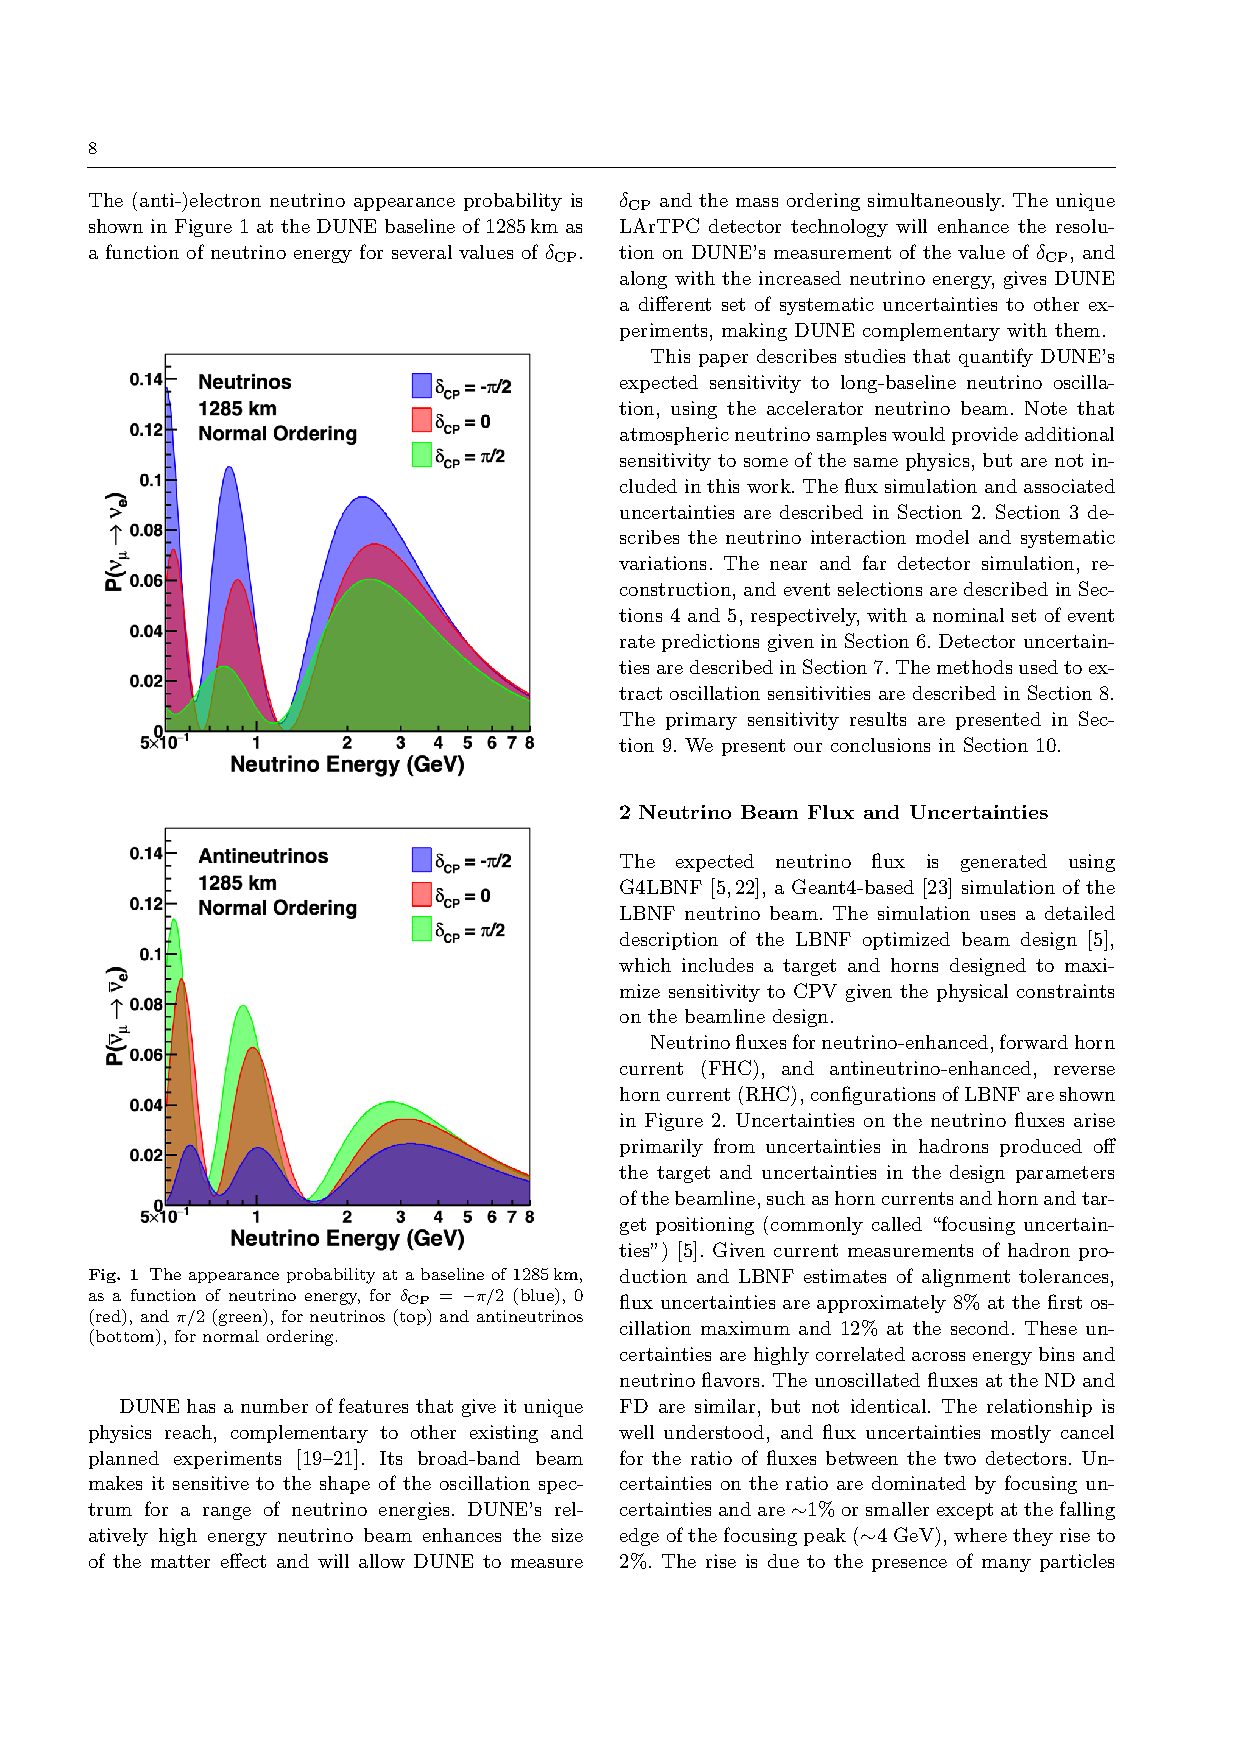
\includegraphics[trim=46bp 466bp 333bp 166bp,clip,width=0.48\textwidth]{dune_appearance_src.pdf}\hfill
    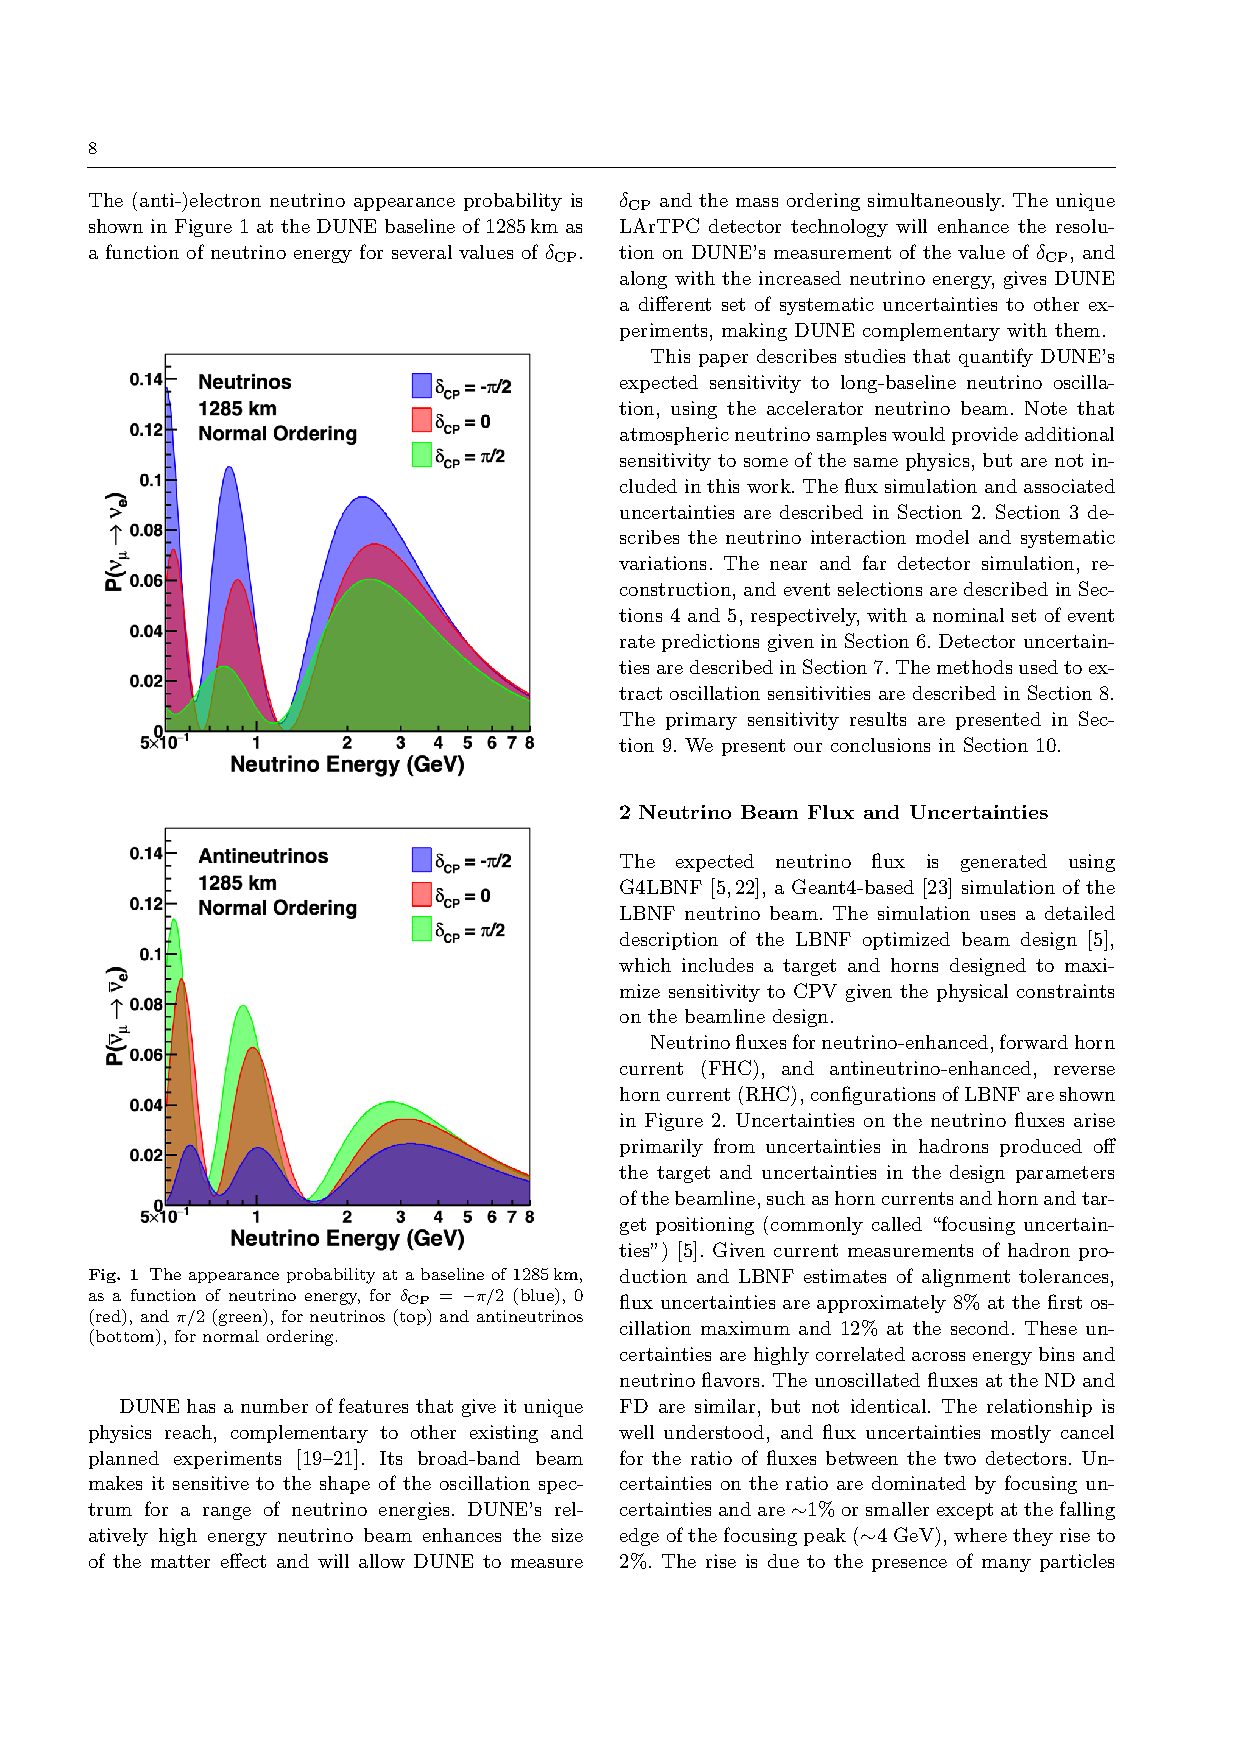
\includegraphics[trim=46bp 238bp 333bp 394bp,clip,width=0.48\textwidth]{dune_appearance_src.pdf}
    \caption{The $\numu\to\nue$ (left) and $\numubar\to\nuebar$ (right) appearance
    probabilities at DUNE's $1285$\,km baseline in the normal ordering, for
    $\dcp=-\pi/2$ (blue), $0$ (red) and $\pi/2$ (green). The first oscillation
    maximum is the broad peak near $2.5$\,GeV; the second is the sharper peak
    near $0.8$\,GeV. Reproduced from the DUNE Collaboration~\citep[Fig.~1, p.~8]{DUNE2020}.}
    \label{fig:dune-appearance}
\end{figure}

DUNE will also measure $\theta_{23}$ with world-leading precision allowing for the octant to be determined and the wide-band beam will allow for the remaining degeneracy between $\dcp$ and $\theta_{23}$ to be resolved~\citep[p.~3]{DUNE2025Science}. With the complementary $\theta_{23}$ dependence of both oscillation channels (Sec.~\ref{sec:three-flavour}), DUNE’s appearance and disappearance measurements together will probe the octant~\citep[p.~28]{DUNE2020}. To achieve the target level of precision, the neutrino--argon cross section as a function of energy must be determined at the few-percent level. This shared cross-section systematic is constrained by the near detector; the DUNE-PRISM system moves the near LArTPC off axis allowing it to sample a range of off-axis energies spectra~\cite{DUNE2025Science}.

\paragraph{Hyper-Kamiokande.}
Hyper-Kamiokande will share the same baseline as T2K but will use a significantly larger water-Cherenkov detector~\cite{HyperK2025}. 
Like with T2K, since the baseline is short, so are the matter effects. The appearance channel therefore doesn't have high ordering 
sensitivity but will primarily measure $\dcp$. The ordering sensitivity will instead arise from atmospheric neutrino, since they 
will feel an enhanced matter effect due to their distances traveled through the Earth. 

Both next generation experiments seek to measure the same parameters, but in different ways, with different detector technologies, baselines and beam energy spectra. Therefore, agreement between them would point towards a correct shared understanding of neutrino oscillations, while disagreement could point towards issues with one of the experiments, or an incomplete three-flavour picture~\citep[p.~3]{DUNE2025Science}.

% ============================================================
\subsection{Current Constraints and Open Questions}
\label{sec:landscape-open}

Table~\ref{tab:osc-params} collects the current parameter values. The global-fit column
is taken from NuFIT~6.1, which combines data available through its November~2025
closing date (including the first JUNO solar-pair result); the second column gives the
leading single-experiment determination for each parameter.

\begin{table}[tb]
    \centering
    \small
    \begin{tabular}{lccll}
        \toprule
        & \multicolumn{2}{c}{NuFIT~6.1 global fit} & \multicolumn{2}{c}{Leading direct} \\
        \cmidrule(lr){2-3}\cmidrule(lr){4-5}
        Parameter & Normal & Inverted & Value & Source \\
        \midrule
        $\sin^{2}\theta_{12}$ & $0.3088^{+0.0067}_{-0.0066}$ & $0.3088^{+0.0067}_{-0.0066}$
            & $0.3092 \pm 0.0087$ & JUNO \\
        $\sin^{2}\theta_{23}$ & $0.470^{+0.017}_{-0.014}$ & $0.550^{+0.013}_{-0.016}$
            & $0.55 \pm 0.02$ & NOvA \\
        $\sin^{2}\theta_{13}$ & $0.02248^{+0.00055}_{-0.00059}$ & $0.02262^{+0.00057}_{-0.00056}$
            & $0.0851 \pm 0.0024$\rlap{$^{\dagger}$} & Daya Bay \\
        $\dcp/^{\circ}$ & $212^{+26}_{-36}$ & $274^{+22}_{-25}$
            & --- & \\
        $\dm{21}/10^{-5}~\text{eV}^{2}$ & $7.537^{+0.094}_{-0.10}$ & $7.537^{+0.094}_{-0.10}$
            & $7.50 \pm 0.12$ & JUNO \\
        $\dm{3\ell}/10^{-3}~\text{eV}^{2}$ & $+2.511^{+0.021}_{-0.020}$ & $-2.483^{+0.020}_{-0.020}$
            & $+2.431^{+0.036}_{-0.034}$ & NOvA \\
        \bottomrule
    \end{tabular}
    \caption{Three-flavour oscillation parameters. Global-fit values are the NuFIT~6.1
    best-fit points with $1\sigma$ uncertainties for the normal (NO) and inverted (IO)
    orderings, from the variant including Super-Kamiokande and IceCube atmospheric
    data~\cite{NuFIT61,NuFIT60}; that analysis closes in November~2025. The final
    columns give the leading single-experiment determination:
    JUNO~\citep[p.~15]{JUNO2026}, NOvA~\citep[p.~2]{NOvA2025} and
    Daya Bay~\cite{DayaBay2023}. Here $\dm{3\ell}$ denotes $\dm{31}$ for the normal and
    $\dm{32}$ for the inverted ordering. $^{\dagger}$Daya Bay reports
    $\sin^{2}2\theta_{13}$ rather than $\sin^{2}\theta_{13}$.}
    \label{tab:osc-params}
\end{table}

Three questions remain open.

\paragraph{The mass ordering.}
The sign of $\dm{32}$ is still open. Fig.~\ref{fig:bievent} shows why a single baseline
cannot separate it from $\dcp$, and the joint T2K--NOvA analysis finds no strong
preference either way~\citep[p.~5]{T2KNOvA2025}.

\paragraph{The $\theta_{23}$ octant.}
Disappearance data constrain $\sin^{2}(2\theta_{23})$ and are therefore blind to the
octant at leading order. Fig.~\ref{fig:nova-contour} shows the present status: NOvA's
allowed region sits almost symmetrically about maximal mixing, which is the hardest case
to resolve.

\paragraph{$\dcp$.}
The value of $\dcp$ is the least well determined of the six parameters. Its allowed range
depends on the assumed ordering, as the joint T2K--NOvA interval already showed, and
Fig.~\ref{fig:bievent} shows why. CP conservation is not yet excluded.

Until DUNE and Hyper-Kamiokande resolve these questions, they must be constrained by the
experiments now running. NOvA's disappearance measurement is the leading direct
determination of $\dm{32}$~\citep[p.~1]{NOvA2025}, and it is that measurement --- the
far-detector spectrum, its systematic treatment and its interpretation --- that the
remainder of this thesis addresses.


\clearpage
% ---- Bibliography ----------------------------------------------------------
\bibliographystyle{unsrtnat}
\bibliography{main}

\end{document}
